\section{ \bfseries Nonlinear Program (NLP)}
A nonlinear program is considered in the form\\
\begin{align*}
&\min_{x} \quad f(x)\tag{5}\label{con:op5.1}\\
& s.t. \quad g(x)=0\\
& \quad \quad  l\le x \le u
\end{align*}
Assuming that the involved functions are sufficiently smooth for the algorithms discussed in this course to work. Assume that $\nabla_{g(x)}$ has full column rank.
%%%%%%%%%%%%%%%%%%%%%%%%%%%%%%%%%%%%%%%%%%
%%%%%%%%%%%%%%%%%%%%%%%%%%%%%%%%%%%%%%%%%%%%%%%%%%%%%%%%%%%%%%%%%%%%%%%%%%%%%%%%%%%%%
%%%%%%%%%%%%%%%%%%%%%%%%%%%%%%%%%%%%%%%%%%%
%%%%%%%%%%%%%%%%%%%%%%%%%%%%%%%%%%%%%%%%%%
%%%%%%%%%%%%%%%%%%%%%%%%%%%%%%%%%%%%%%%%%%%
\subsection{\bfseries Lagrangian function}
\begin{shaded}
{ Question: What is the Lagrangian function for this problem?}
\end{shaded}
First, the  nonlinear program problem (\ref{con:op5.1}) can be equivalent to the inequailty constrained form

\begin{align*}
&\min_{x} \quad f(x) \tag{5.1}\label{con:op5.2}\\
& s.t. \quad g(x)=0\\
& \quad \quad  h(x)=\begin{bmatrix}
x-l \\ u-x\end{bmatrix}=\left[I\quad -I\right]^{\prime}x+\begin{bmatrix}
-l \\ u\end{bmatrix}\ge 0\Leftrightarrow h(x) \ge 0
\end{align*}\\[0.3cm]
Lagrangian function\\
$$L(x, \mu, \lambda)=f(x)-\mu^{\prime}g(x) -\lambda^{\prime}h(x) \eqno{(5.2)}$$
%%%%%%%%%%%%%%%%%%%%%%%%%%%%%%%%%%%%%%%%%%
%%%%%%%%%%%%%%%%%%%%%%%%%%%%%%%%%%%%%%%%%%%
%%%%%%%%%%%%%%%%%%%%%%%%%%%%%%%%%%%%%%%%%%
%%%%%%%%%%%%%%%%%%%%%%%%%%%%%%%%%%%%%%%%%%%
%%%%%%%%%%%%%%%%%%%%%%%%%%%%%%%%%%%%%%%%%%
%%%%%%%%%%%%%%%%%%%%%%%%%%%%%%%%%%%%%%%%%%%
\newpage
\subsection{\bfseries Necessary optimality conditions}
\begin{shaded}
{Question: What is the necessary first order optimality conditions for the nonlinear program?}
\end{shaded}
First the gradient of the Lagrangian function is
$$\nabla_{x} L(x, \mu, \lambda)=\nabla f(x)-\nabla g(x) \mu-\nabla h(x) \lambda\eqno{(5.3)}$$
From the question it is shown that the $\nabla_{g(x)}$ has full column rank and the inequlity form is $l\le x \le u$ so the assumption of LICQ is valid. Assuming that $\nabla_{g_i(x)}$ and $\nabla_{h_i(x)}$ are linearly independent for all $i \in \mathcal{A}(x)$. \\
The necessary first order optimality conditions\\[0.3cm]
Let $x$ be a local minimizer then
\begin{align*}
    \nabla_{x} L(x, \mu, \lambda)&=\nabla f(x)-\nabla g(x) \mu-\nabla h(x) \lambda=0\tag{5.4}\\
    g(x)&=0\tag{5.5}\\
    h(x)&\ge 0\tag{5.6}\\
    \lambda&\ge 0\tag{5.7}\\
    \lambda h(x)&=0\tag{5.8}
\end{align*}

%%%%%%%%%%%%%%%%%%%%%%%%%%%%%%%%%%%%%%%%%%
%%%%%%%%%%%%%%%%%%%%%%%%%%%%%%%%%%%%%%%%%%%
%%%%%%%%%%%%%%%%%%%%%%%%%%%%%%%%%%%%%%%%%%
%%%%%%%%%%%%%%%%%%%%%%%%%%%%%%%%%%%%%%%%%%%
%%%%%%%%%%%%%%%%%%%%%%%%%%%%%%%%%%%%%%%%%%
%%%%%%%%%%%%%%%%%%%%%%%%%%%%%%%%%%%%%%%%%%%
\subsection{\bfseries Sufficient optimality conditions}
\begin{shaded}
{Question:What are the sufficient second order optimality conditions for the nonlinear program?}
\end{shaded}
First the feasible active direction $h$ is defined. Let $x$ be any feasible point. Then any non-zero vector, $h$, is a feasible active direction if
\begin{align*}
    \nabla g_i(x)^{\prime}h&=0 \qquad \forall i \in \mathcal{A}(x)\tag{5.9}\\
    \nabla h_i(x)^{\prime}h&=0 \quad \text{and} \quad  \lambda_i>0 \qquad \forall i \in \mathcal{A}(x)\tag{5.10}\\
\end{align*}
Then assuming that $(x,\lambda)$ satisfy the first order KKT conditions. If for all feasible active directions, $h \neq 0 $,
$$h^{\prime}\nabla_{xx}^2L(x,\mu,\lambda)h>0\eqno{(5.11)}$$
Then it can be said that the $x$ is a strict local constrained minimizer.
%%%%%%%%%%%%%%%%%%%%%%%%%%%%%%%%%%%%%%%%%%
%%%%%%%%%%%%%%%%%%%%%%%%%%%%%%%%%%%%%%%%%%%
%%%%%%%%%%%%%%%%%%%%%%%%%%%%%%%%%%%%%%%%%%
%%%%%%%%%%%%%%%%%%%%%%%%%%%%%%%%%%%%%%%%%%%
%%%%%%%%%%%%%%%%%%%%%%%%%%%%%%%%%%%%%%%%%%
%%%%%%%%%%%%%%%%%%%%%%%%%%%%%%%%%%%%%%%%%%%
\subsection{\bfseries Description of test problem}
\begin{shaded}
{Question:Choose a specific test problem for a nonlinear program in the form. Present
the problem and argue why you chose this problem.}
\end{shaded}
The Himmelblau Optimization Problem is considered
\begin{align*}
    \min_x \quad &f(x)=\left(x_1^2+x_2-11\right)^2+\left(x_1+x_2^2-7\right)^2\tag{5.12}\\
    &g(x)=\left(x_1+2\right)^2-x_2= 0\\
    &h_1(x)=-x_1+3\ge 0\\
    &h_2(x)=x_2+2\ge 0\\
\end{align*}
There are several reasons to choose the Himmelblau Optimization Problem. First,  the objective function is continuous as required. This function is not convex and has four local minima at 
$$\begin{array}{l}
f\left(\mathbf{x}^{*}\right)=0 \text { at } \mathbf{x}^{*}=(3,2) \\
f\left(\mathbf{x}^{*}\right)=0 \text { at } \mathbf{x}^{*}=(-2.805118,3.283186) \\
f\left(\mathbf{x}^{*}\right)=0 \text { at } \mathbf{x}^{*}=(-3.779310,-3.283186) \\
f\left(\mathbf{x}^{*}\right)=0 \text { at } \mathbf{x}^{*}=(3.584458,-1.848126)
\end{array}$$
Because the SQP algorithm tested is based on iteration, different stating points can be chose to test the optimization results. In order to conveniently present the iterative trajectory of points in the contour, this problem which is defined on the 2-dimensional space is chosen for the test.
The contour of the function is showed here
\begin{figure}[H]
\centering
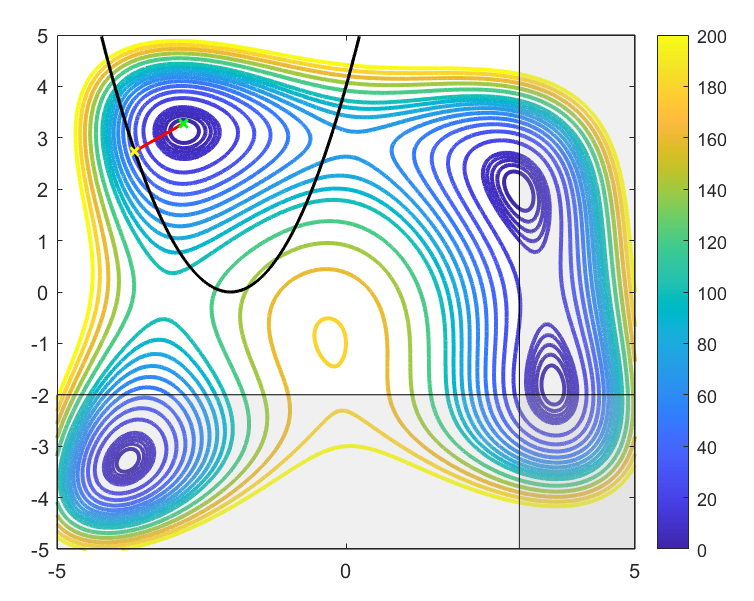
\includegraphics[scale=0.5]{figures/HB_map1.PNG}
\caption{The contour of the function in $x_1\in[-5, 5],x_2\in[-5,5]$}
\label{fig:labe5.4.1}
\end{figure}
A more specific contour under inequality conditions($-x_1+3\ge 0$,$x_2+2\ge 0$)
\begin{figure}[H]
\centering
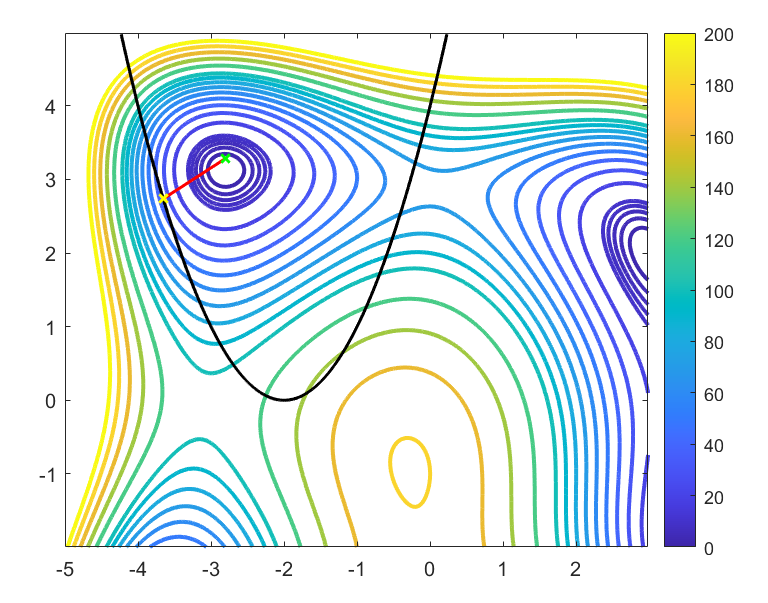
\includegraphics[scale=0.5]{figures/HB_map_ieq.PNG}
\caption{The contour of the function in $x_1\in[-5, 3],x_2\in[-2,5]$}
\label{fig:labe5.4.2}
\end{figure}
The black curve is the equality constraint $\left(x_1+2\right)^2-x_2= 0$, and one of the two ends of the red line is the minimum point($-2.8051,3.2832$) of the objective equation without constraints, corresponding to the green $\times$, and the other is the minimum point($-3.6546,2.7377$) under the constraints of the equations and inequalities of this problem, corresponding to the yellow $\times$.

%%%%%%%%%%%%%%%%%%%%%%%%%%%%%%%%%%%%%%%%%%
%%%%%%%%%%%%%%%%%%%%%%%%%%%%%%%%%%%%%%%%%%%
%%%%%%%%%%%%%%%%%%%%%%%%%%%%%%%%%%%%%%%%%%
%%%%%%%%%%%%%%%%%%%%%%%%%%%%%%%%%%%%%%%%%%%
%%%%%%%%%%%%%%%%%%%%%%%%%%%%%%%%%%%%%%%%%%
%%%%%%%%%%%%%%%%%%%%%%%%%%%%%%%%%%%%%%%%%%%
\subsection{\bfseries Solution to the problem by fmincon}
\begin{shaded}
{Question:Solve the test problem using a library function for nonlinear programs, e.g. fmincon in Matlab.}
\end{shaded}
First, it is necessary to respectively construct the function that outputs the objective function and his gradient, and the function that outputs the equality and inequality constraints and his gradient.\\[0.3cm]
For objective function and his gradient
\begin{align*}
    f(x_1,x_2)&=\left(x_1^2+x_2-11\right)^2+\left(x_1+x_2^2-7\right)^2\\
    \nabla f(x)&=\left[\begin{array}{l}
4 x_{1}\left(x_{1}^{2}+x_{2}-11\right)+2\left(x_{1}+x_{2}^{2}-7\right) \\
2\left(x_{1}^{2}+x_{2}-11\right)+4 x_{2}\left(x_{1}+x_{2}^{2}-7\right)
\end{array}\right]\tag{5.13}
\end{align*}
{\setmainfont{Courier New Bold} \scriptsize         
\begin{lstlisting}
function [f,dfdx]=objfunHimmelblau(x,p)
tmp1=x(1)*x(1)+x(2)-11;
tmp2=x(1)+x(2)*x(2)-7;
f=tmp1*tmp1+tmp2*tmp2;

%compute gradient
if nargout>1
    dfdx=zeros(2,1);
    dfdx(1,1)=4*tmp1*x(1)+2*tmp2;
    dfdx(2,1)=2*tmp1+4*tmp2*x(2);
end
\end{lstlisting}}
For equality constraints and its gradient
\begin{align*}
c_1(x_1,x_2)&=\left(x_1+2\right)^2-x_2\\
\nabla c_1(x)&=\left[\begin{array}{c}
2\left(x_{1}+2\right) \\
-1
\end{array}\right]\tag{5.14}
\end{align*}
{\setmainfont{Courier New Bold} \scriptsize         
\begin{lstlisting}
function [c,ceq,dcdx,dceqdx]=confunHimmeblau(x,p)
c=zeros(0,1);
ceq=zeros(1,1);
%c<=0  
x1=x(1,1);
x2=x(2,1);
tmp=x1+2;
%Equality constraint 
ceq=tmp^2-x2;

% computer constraint gradients
if nargout>2
    dcdx=zeros(2,0);
    dceqdx=zeros(2,1);
    %Gradient of Equality constraint
    dceqdx(1,1)=2*tmp;
    dceqdx(2,1)=-1;
end
\end{lstlisting}}
Four starting points that are located on the left A=($-5,3$), below B=($-2,-2$), right C=($3,3$), and above D=($-2,5$) of the equality constraint curve (position in the figure) and at inequality constraint and the intersection E=($3,-2$) of two inequality constraints are selected . Please see the driver files in Appendix \ref{6.5.1}, \ref{6.5.2} and \ref{6.5.3}. The SQP algorithm and interior-point algorithm are both tested by fmincon, and the result is 
\begin{table}[!htbp]
\centering
\begin{tabular}{|c|c|c|c|c|c|}
\hline
&A($-5,3$)&B($-2,-2$)&C($3,3$)&D($-2,5$)&E($3,-2$)\\
\hline
SQP&($-3.65,2.73$)&($-3.65,2.73$)&($-0.29,2.89$)&($-3.65,2.73$)&($-0.29,2.89$)\\
\hline
Interior-point&($-3.65,2.73$)&($-3.65,2.73$)&($-0.29,2.89$)&($-3.65,2.73$)&($-0.29,2.89$)\\
\hline
\end{tabular}
\end{table}
$$\begin{array}{l}
f\left(\mathbf{x}^{*}\right)=65.43 \text { at } \mathbf{x}^{*}=(-0.29,2.89) \\
f\left(\mathbf{x}^{*}\right)=35.93 \text { at } \mathbf{x}^{*}=(-3.65,2.73) \\
\end{array}$$
It is found that whether the algorithm SQP or Interior-point in the fmincon function is used, the minimum value obtained for the same starting point is the same. It can be seen that starting points $A$, $B$, and $D$ have reached the correct minimum points, but starting points $C$ and $E$ reached a sub-minimum point.\\
First iterative trajectory of starting points $C$ and $E$ in the contour is showed 
\begin{figure}[H]
\centering
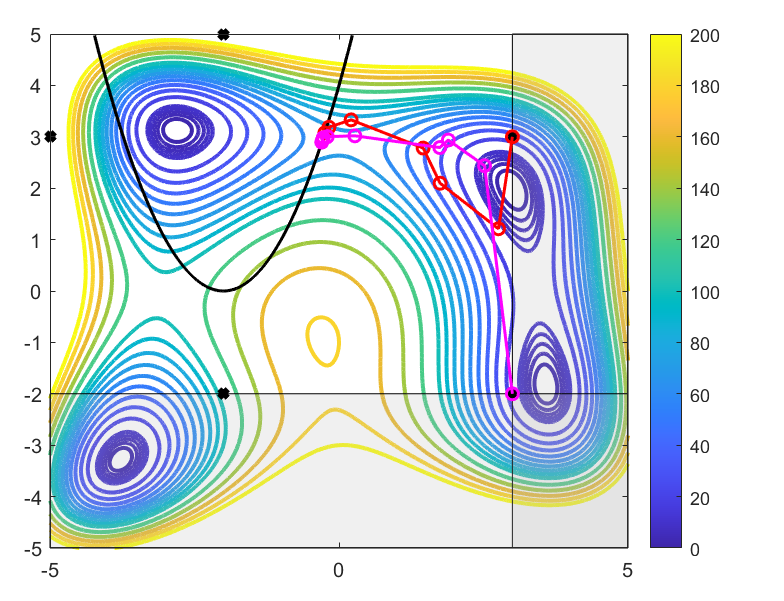
\includegraphics[scale=0.5]{figures/fmincon_CE.PNG}
\caption{Iterative trajectory of starting points $C$ and $E$}
\label{fig:labe5.4.3}
\end{figure}
It is found that because there is a maximum value in the lower part of the equation constraint curve, when the starting point is on the right side of the equation constraint curve, the iteration point will not cross the maximum value area, but in the right half of the equation constraint curve to search for the minimum point. As a result, the correct minimum value cannot be found in the left half of the equality constraint, but can only reach the sub-minimum value.
Iterative trajectory of starting points $A$, $B$, and $D$ in the contour is showed 
\begin{figure}[H]
\centering
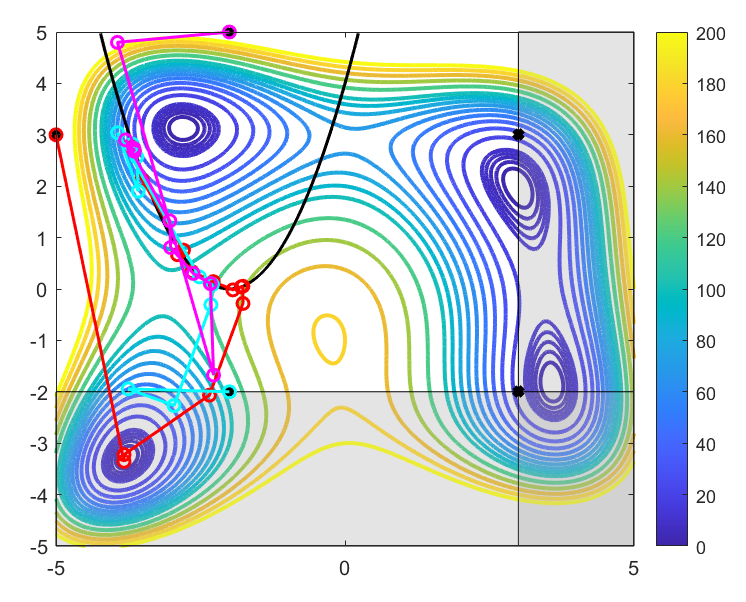
\includegraphics[scale=0.5]{figures/fmincon_ABD.PNG}
\caption{Iterative trajectory of starting points $A$, $B$, and $D$}
\label{fig:labe5.4.4}
\end{figure}
When the starting point is not obstructed by the area where the maximum value is, the correct minimum point can be found.
%%%%%%%%%%%%%%%%%%%%%%%%%%%%%%%%%%%%%%%%%%
%%%%%%%%%%%%%%%%%%%%%%%%%%%%%%%%%%%%%%%%%%%
%%%%%%%%%%%%%%%%%%%%%%%%%%%%%%%%%%%%%%%%%%
%%%%%%%%%%%%%%%%%%%%%%%%%%%%%%%%%%%%%%%%%%%
%%%%%%%%%%%%%%%%%%%%%%%%%%%%%%%%%%%%%%%%%%
%%%%%%%%%%%%%%%%%%%%%%%%%%%%%%%%%%%%%%%%%%%
\newpage
\subsection{\bfseries SQP algorithm with damped BFGS}
\begin{shaded}
{Question:Explain, discuss and implement an SQP procedure with a damped BFGS approximation to the Hessian matrix for the problem. Make a table with the iteration sequence for different starting points. Plot the iteration sequence in a
contour plot. Discuss the results.}
\end{shaded}
First, the KKT conditions of this nonlinear problem are considered
\begin{align*}
\nabla_x L(x,\mu,\lambda)&=\nabla f(x)-\nabla g(x)\mu-\nabla h(x) \lambda=0\tag{5.15}\\
\nabla_{\mu} L(x,\mu,\lambda)&=-g(x)=0\tag{5.16}\\
\nabla_{\lambda} L(x,\mu,\lambda)&=-h(x)\le 0\tag{5.17}
\end{align*}
Newton's method 

$$\left[\begin{array}{cc}
\nabla_{x x}^{2} L\left(x_{k}, \mu_{k}, \lambda_{k}\right) & -\nabla g\left(x_{k}\right) \\
-\nabla g\left(x_{k}\right)^{\prime} & 0
\end{array}\right]\left[\begin{array}{c}
\Delta x \\
\Delta \mu
\end{array}\right]=-\left[\begin{array}{c}
\nabla_{x} L\left(x_{k}, \mu_{k}, \lambda_{k}\right) \\
-g\left(x_{k}\right)
\end{array}\right]\eqno{(5.18)}$$\\
$$\left[-\nabla h(x_k)^{\prime}\right]\left[\Delta \lambda\right]\le -\left[-h(x_k)\right]\eqno{(5.19)}$$
The assumption is noted that first the constraint Jacobian $\nabla g(x_k)$ has full column rank, and the matrix $L\left(x_{k}, \mu_{k}, \lambda_{k}\right) & -\nabla g\left(x_{k}\right)$ is positive definite on the tangent space of the constraints, that is, $d^{\prime}L\left(x_{k}, \mu_{k}, \lambda_{k}\right) & -\nabla g\left(x_{k}\right)d> 0$ for all $d\noq 0$ such that $\nabla dg(x_k)=0$
Then a subproblem which is a quadratic programming problem can be constructed
$$\begin{aligned}
\min _{\Delta x \in \mathbb{R}^{n}} \qquad & \frac{1}{2} \Delta x^{\prime}\left[\nabla_{x x}^{2} L\left(x_{k}, \mu_{k},\lambda_{k}\right)\right] \Delta x+\left[\nabla_{x} L\left(x_{k}, \mu_{k},\lambda_{k}\right)\right]^{\prime} \Delta x \\
\text {s.t.} \qquad & \nabla g\left(x_{k}\right)^{\prime} \Delta x=-g\left(x_{k}\right)\\
& \nabla h\left(x_{k}\right)^{\prime} \Delta x\ge -h\left(x_{k}\right)
\end{aligned}\eqno{(5.20)}$$
Which can be expressed as
$$\begin{aligned}
\min _{\Delta x \in \mathbb{R}^{n}} \qquad & \frac{1}{2} \Delta x^{\prime}H\Delta x+g^{\prime}\Delta x \\
\text {s.t.} \qquad & A^{\prime} \Delta x=b\\
& C^{\prime} \Delta x=d
\end{aligned}\eqno{(5.21)}$$
with
$$\begin{array}{lll}
H=\nabla_{x x}^{2} L\left(x_{k}, \mu_{k},\lambda_{k}\right) & g=\nabla f\left(x_{k}\right)\\
A=\nabla g\left(x_{k}\right) & b=-h\left(x_{k}\right)\\
C=\nabla g\left(x_{k}\right) & d=-h\left(x_{k}\right)
\end{array}$$
The Hessian matrix of the nonlinear function is always hard to compute, so the damped BFGS approximation to the Hessian matrix is always used. The idea is to update a $B_k$ to replace the $H$, where the vectors $s_k$ and $y_k$ are defined as 
\begin{align*}
    s_k&=x_{k+1}-x_k\tag{5.22}\\
    y_k&=\nabla_{x} L\left(x^{k+1},\mu^{k+1},\lambda^{k+1}\right)-\nabla_{x}L\left(x^{k}, \mu^{k+1},\lambda^{k+1}\right)\tag{5.23}
\end{align*}
Given a symmetric and positive definite matrix $B_k$\\
Defined $r_k$ as
$$r_{k}=\theta_{k} y_{k}+\left(1-\theta_{k}\right) B_{k} s_{k}\eqno{(5.24)}$$
Where the scalar $\theta_{k}$ is defined as
$$\theta_{k}=\left\{\begin{array}{ll}
1 & \text {if } s_{k}^{\prime} y_{k} \geq 0.2 s_{k}^{\prime} B_{k} s_{k} \\
\left(0.8 s_{k}^{\prime} B_{k} s_{k}\right) /\left(s_{k}^{\prime} B_{k} s_{k}-s_{k}^{\prime} y_{k}\right) & \text { if } s_{k}^{\prime} y_{k}<0.2 s_{k}^{\prime} B_{k} s_{k}
\end{array}\right\eqno{(5.25)}$$
Update $B_k$ as follows
$$B_{k+1}=B_{k}-\frac{B_{k} s_{k} s_{k}^{\prime} B_{k}}{s_{k}^{\prime} B_{k} s_{k}}+\frac{r_{k} r_{k}^{\prime}}{s_{k}^{\prime} r_{k}}\eqno{(5.26)}$$
From the updating with $r_k$ replaced by $r_k$. It guarantees that $B_{k+1}$ is positive definite.

{\setmainfont{Times New Roman}\bfseries Pseudo-code}
\begin{algorithm}[H]
	\caption{ SQP algorithm with damped BFGS}
	\begin{algorithmic}[1]
	    \STATE Given a starting point($x_0,\mu_0,\lambda_0$), set $k=0$\\
		\STATE Evaluate $f_0,\nabla f_0,g_0,\nabla g_0,h_0,\nabla h_0$\\
		\STATE Choose an initial $n \times n$ symmetric positive definite Hessian approximation $B_0$, always an Identity matrix\\
        \WHILE {(not converged)}\\
		\STATE Compute the $p_k$($\Delta x_k$),$\mu_{k+1}$ and $\lambda_{k+1}$by solving the sub-quadratic-problem\\
		\STATE Compute $x_{k+1}=x_k+p_k$\\
		\STATE Compute $\nabla_{x}L\left(x_{k}, \mu_{k+1},\lambda_{k+1}\right)=\nabla f(x_k)-\nabla g(x_k)\mu_{k+1}-\nabla h(x_k)\lambda_{k+1}$\\
		\STATE Evaluate $f_{k+1},\nabla f_{k+1},g_{k+1},\nabla g_{k+1},h_{k+1},\nabla h_{k+1}$\\
		\STATE Compute $\nabla_{x}L\left(x_{k+1}, \mu_{k+1},\lambda_{k+1}\right)=\nabla f(x_{k+1})-\nabla g(x_{k+1})\mu_{k+1}-\nabla h(x_{k+1})\lambda_{k+1}$\\
		\STATE Compute the $s_k$ and $y_k$\\
		\STATE Update the Hessian matrix by the modified BFGS procedure\\
		\STATE $k=k+1$\\
		\ENDWHILE
    \end{algorithmic}
\end{algorithm}
Next the specific Matlab code of implementation is showed. The function "Hg_f" which calculate the gradients and hessian of object-function and itself, the "Hg_ceq" which calculate the gradients and hessian of equality constraints and itself, the "Hg_ciq" which calculate the gradients and hessian of equality constraints and itself ,the "Qpsolver_Sqp" which solve the sub-problem of SQP algorithm are stated in appendix \ref{6.5.4}, \ref{6.5.5}, \ref{6.5.6} and \ref{6.5.7}. Only the main program is showed here\\

{\setmainfont{Courier New Bold} \scriptsize         
\begin{lstlisting}
function [x,output]=Sqp_Bfgs(x0,lam_eq0,lam_ineq0)
% Sqp_Bfgs  SQP algorithm with damped BFGS and line search
%
%          min  f(x)
%           x
%          s.t. ceq(x)=0  (Lagrange multiplier lam_eq)    
%               ciq(x)>=0  (Lagrange multiplier lam_ineq)  
% Syntax: [x,output]=Sqp_Bfgs(x0,lam_eq0,lam_ineq0)
%         output.fval: minimum value
%         output.dL: convergence of delta_L
%         output.ceq: convergence of ceq
%         output.Xarray=Xarray: Iteration trajectory  
epsilon=1e-6;

Xarray=[];
normdLarray=[];
normceqarray=[];
Xarray=[Xarray x0];

nx=size(x0,1);
Bk=eye(nx);
%evaluate the gradient
[~,df,~]=Hg_f(x0);
[ceq,dceq,~]=Hg_ceq(x0);
[ciq,dciq,~]=Hg_ciq(x0);
xk=x0;
lam_eqk=lam_eq0;
lam_ineqk=lam_ineq0;
iteration=0;
iteration_max=200;
while(iteration<iteration_max)
    %Solve the subproblem(QP)
    [p,lameq,lamineq]=Qpsolver_Sqp(Bk,df,dceq,ceq,dciq,ciq);
    %Take step and update x(k+1),lameq(k+1),lamineq(k+1)
    xk=xk+p;
    lam_eqk=-lameq;
    lam_ineqk=-lamineq;
    %Calculate dL(k) with x(k) and lameq(k+1),lamineq(k+1)
    Lk=df-dceq.*lam_eqk-dciq*lam_ineqk;
    %Re-evaluate
    [~,df,~]=Hg_f(xk);
    [ceq,dceq,~]=Hg_ceq(xk);
    [ciq,dciq,~]=Hg_ciq(xk);
    %Calculate L(k+1) with x(k+1) and lam(k+1)
    Lk2=df-dceq.*lam_eqk-dciq*lam_ineqk;
    %Damped BFGS update
    pk=p;
    qk=Lk2-Lk;
    judge=(pk'*qk>=0.2*pk'*(Bk*pk));
    thetak=judge.*1+(~judge).*((0.8*pk'*(Bk*pk))/(pk'*(Bk*pk)-pk'*qk));
    rk=thetak*qk+(1-thetak)*(Bk*pk);
    Bk=Bk-((Bk*pk)*(pk'*Bk))/(pk'*(Bk*pk))+(rk*rk')/(pk'*rk);
    %Check teh convergence
    if ((norm(Lk2,"inf")<epsilon)&&(norm(ceq,"inf")<epsilon)&&(max(abs(ciq)) + epsilon >= 0)...
       &&(min(lam_ineqk) + epsilon >= 0))
        break;
    end
    iteration=iteration+1;
    Xarray=[Xarray xk];
    normdLarray=[normdLarray norm(Lk2,"inf")];
    normceqarray=[normceqarray norm(ceq,"inf")];
end
[fval,~,~]=Hg_f(xk);
x=xk;
output.fval=fval;
output.xarray=Xarray;
output.dL=normdLarray;
output.ceq=normceqarray;
output.iteration=iteration;
end
\end{lstlisting}}
The algorithm will be tested with the same initial
points as in the section 5.5. Please see the test code in Appendix \ref{6.5.8}. Iterative trajectory of starting points $A$, $B$, $C$, $D$ and $E$ in the contour is showed 

\begin{figure}[H]
\centering
\setlength{\abovecaptionskip}{0cm} 
\setlength{\belowcaptionskip}{-0.5cm}
\subfigure[$A(-5,3)$]{
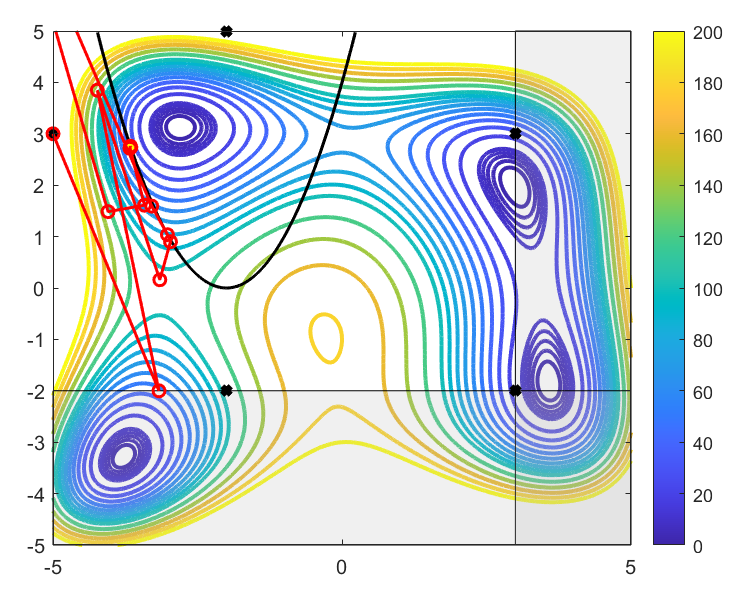
\includegraphics[scale=0.4]{figures/SQP_BFGS_A.PNG}
%\caption{fig1}
}
\quad
\subfigure[$B(-2,-2)$]{
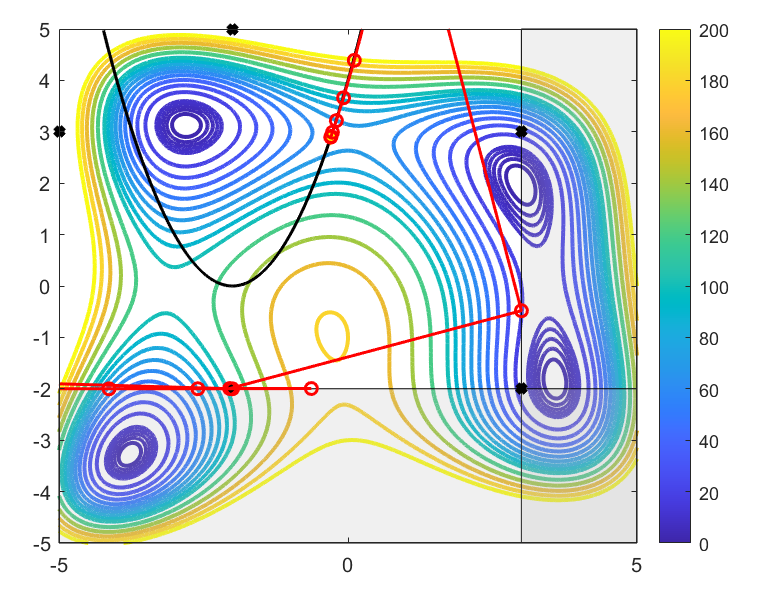
\includegraphics[scale=0.4]{figures/SQP_BFGS_B.PNG}
}
\quad
\subfigure[$C(3,3)$]{
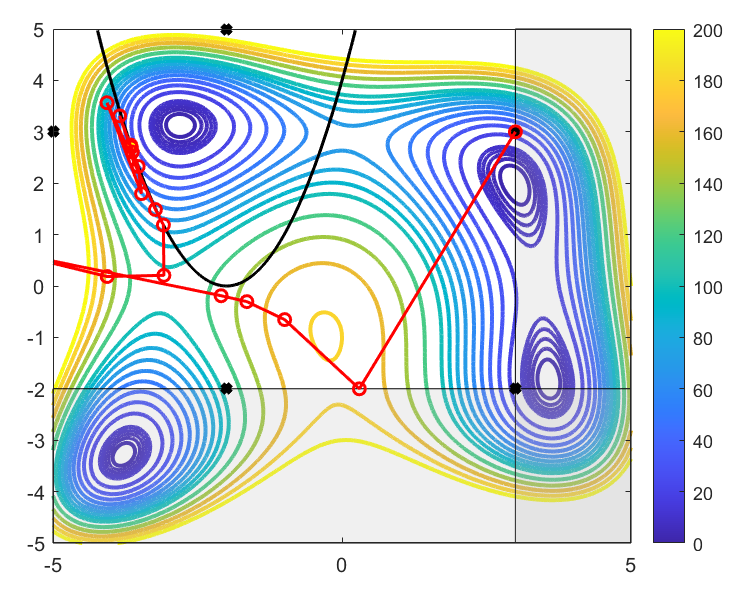
\includegraphics[scale=0.4]{figures/SQP_BFGS_C.PNG}
}
\quad
\subfigure[$D(-2,5)$]{
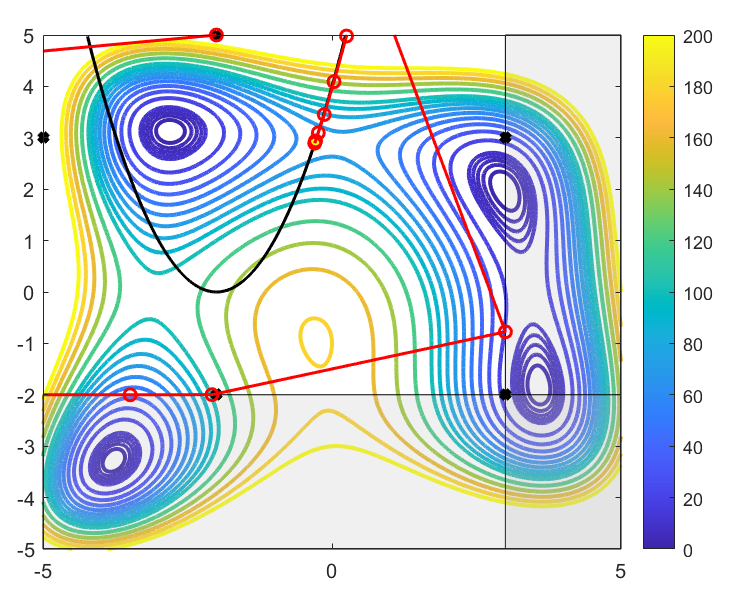
\includegraphics[scale=0.4]{figures/SQP_BFGS_D.PNG}
}
\quad
\subfigure[$E(3,-2)$]{
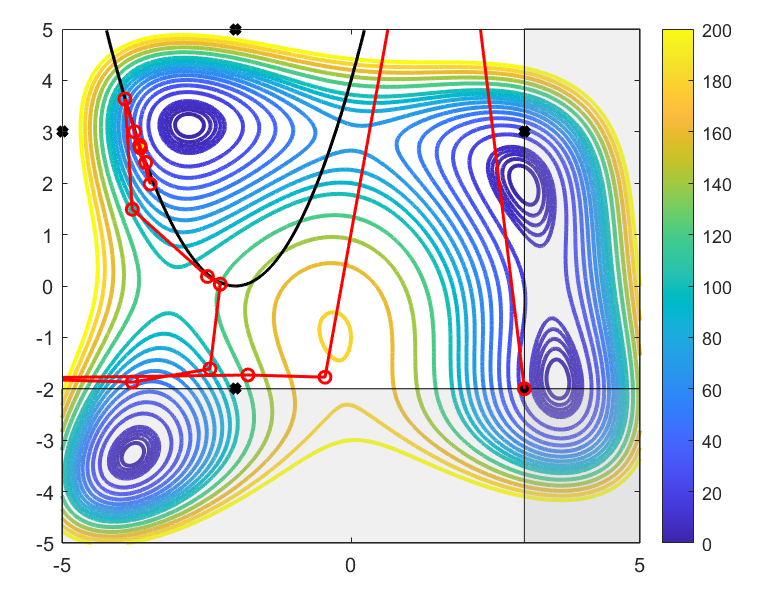
\includegraphics[scale=0.4]{figures/SQP_BFGS_E.PNG}
}
\caption{ Iterative trajectory in contour}
\end{figure}
%%%%%%%%%%%%%%%%%%%%%%%%%%%%%%%%%%%%%%%%%%%%%%%%%%%%%%%
The iteration of table is showed here separately
%%%%%%%%%%%%%%%%%%%%%%%%%%%%%%%%%%%%%%%%%%%%%%%%%%%%%%
\begin{table}[H]
\centering
\setlength{\abovecaptionskip}{0cm} 
\setlength{\belowcaptionskip}{-0.5cm}
\scriptsize
\begin{tabular}{|c|c|c|c|c|c|c|c|c|c|c|}
\hline
$x_0=A(-5,3)$&0&1&2&3&4&5&6&7&8&9\\
\hline
$x_1$&-5.0 & -3.17 & -4.23 & -3.15 & -2.97 & -3.02 & -3.29 & -5.69 & -4.05& -3.42\\
\hline
$x_2$&3.0 & -2.0 & 3.85 & 0.16 & 0.901 & 1.04 & 1.59 & 7.87 & 1.49 & 1.61
\\
\hline
\end{tabular}
\begin{tabular}{|c|c|c|c|c|}
\hline
$x_0=A(-5,3)$&10&11&12&13\\
\hline
$x_1$ & -3.67 & -3.66 & -3.65 & -3.65\\
\hline
$x_2$ & 2.72 & 2.76 & 2.73 & 2.74
\\
\hline

\end{tabular}
\caption{$x_0=A(-5,3)$}
\end{table}

%%%%%%%%%%%%%%%%%%%%%%%%%%%%%%%%%%%%%%%%%%%%%%%%%%%%%%%%%
\begin{table}[H]
\centering
\setlength{\abovecaptionskip}{0cm} 
\setlength{\belowcaptionskip}{-0.5cm} 
\scriptsize
\begin{tabular}{|c|c|c|c|c|c|c|c|c|c|c|}
\hline
$x_0=B(-2,-2)$&0&1&2&3&4&5&6&7&8&9\\
\hline
$x_1$&-2.0 & -64.0 & -33.0 & -21.3 & -11.6 & -6.69 & -4.13 & -2.6 & -0.635 & -2.05 \\
\hline
$x_2$&-2.0 & 0 & -2.0 & 236.0 & -2.0 & -2.0 & -2.0 & -2.0 & -1.99 & -1.99    
\\
\hline
\end{tabular}

\begin{tabular}{|c|c|c|c|c|c|c|c|c|c|c|}
\hline
$x_0=B(-2,-2)$&10&11&12&13&14&15&16&17&18&19\\
\hline
$x_1$&3.0 & 1.22 & 0.972 & 0.955 & 0.902 & 0.663 & 0.347 & 0.109 & -0.0775 & -0.202   \\
\hline
$x_2$&-0.481 & 7.22 & 8.77 & 8.73 & 8.42 & 7.03 & 5.41 & 4.39 & 3.66 & 3.22
\\
\hline
\end{tabular}

\begin{tabular}{|c|c|c|c|c|C|}
\hline
$x_0=B(-2,-2)$&20&21&22&23&24\\
\hline
$x_1$&-0.269 & -0.294 & -0.298 & -0.298 & -0.298  \\
\hline
$x_2$& 2.99 & 2.91 & 2.9 & 2.9 & 2.9
\\
\hline
\end{tabular}
\caption{$x_0=B(-2,-2)$}
\end{table}
%%%%%%%%%%%%%%%%%%%%%%%%%%%%%%%%%%%%%%%%%%%%%%%%%%%%%%%%%%%%%
\begin{table}[H]
\centering
\setlength{\abovecaptionskip}{0cm} 
\setlength{\belowcaptionskip}{-0.5cm}
\scriptsize
\begin{tabular}{|c|c|c|c|c|c|c|c|c|c|c|}
\hline
$x_0=C(3,3)$&0&1&2&3&4&5&6&7&8&9\\
\hline
$x_1$&3.0 & 0.3 & -0.992 & -1.65 & -2.09 & -6.08 & -4.06 & -3.08 & -3.09 & -3.23 \\
\hline
$x_2$&3.0 & -2.0 & -0.654 & -0.304 & -0.189 & 0.737 & 0.184 & 0.208 & 1.19 & 1.49
\\
\hline
\end{tabular}
\begin{tabular}{|c|c|c|c|c|c|c|c|c|c|}
\hline
$x_0=C(3,3)$&10&11&12&13&14&15&16&17&18\\
\hline
$x_1$ &-4.07 & -3.47 & -3.53 & -3.85 & -3.63 & -3.64 & -3.66 & -3.65 & -3.65\\
\hline
$x_2$ & 3.57 & 1.8 & 2.33 & 3.31 & 2.61 & 2.7 & 2.74 & 2.74 & 2.74
\\
\hline

\end{tabular}
\caption{$x_0=C(3,3)$}
\end{table}
%%%%%%%%%%%%%%%%%%%%%%%%%%%%%%%%%%%%%%%%%%%%%%%%%%%%%%%%%%%%%%%
\begin{table}[H]
\centering
\scriptsize
\begin{tabular}{|c|c|c|c|c|c|c|c|c|c|c|}
\hline
$x_0=D(-2,5)$&0&1&2&3&4&5&6&7&8&9\\
\hline
$x_1$&-2.0 & -50.0 & -26.0 & -16.9 & -9.37 & -5.55 & -3.49 & -2.08 & 3.0 & 1.02  \\
\hline
$x_2$&5.0 & 0 & -2.0 & 138.0 & -2.0 & -2.0 & -2.0 & -2.0 & -0.774 & 5.18 
\\
\hline
\end{tabular}
\begin{tabular}{|c|c|c|c|c|c|c|c|c|c|c|c|}
\hline
$x_0=D(-2,5)$&10&11&12&13&14&15&16&17&18&19&20\\
\hline
$x_1$ &0.652 & 0.622 & 0.551 & 0.252 & 0.0345 & -0.134 & -0.237 & -0.285 & -0.297 & -0.298    & -0.298\\
\hline
$x_2$& 6.9 &6.88 & 6.5 & 4.98 & 4.09 & 3.45 & 3.1 & 2.94 & 2.9 & 2.9     & 2.9
\\
\hline

\end{tabular}
\caption{$x_0=D(-2,5)$}
\end{table}
%%%%%%%%%%%%%%%%%%%%%%%%%%%%%%%%%%%%%%%%%%%%%%%%%%%%%%%%%%%
\begin{table}[H]
\centering
\setlength{\abovecaptionskip}{0cm} 
\setlength{\belowcaptionskip}{-0.5cm}
\scriptsize
\begin{tabular}{|c|c|c|c|c|c|c|c|c|c|c|}
\hline
$x_0=E(3,-2)$&0&1&2&3&4&5&6&7&8&9\\
\hline
$x_1$&3.0 & 1.59 & -0.45 & -1.78 & -6.03 & -3.78 & -2.44 & -2.26 & -2.48 & -3.78  \\
\hline
$x_2$&-2.0 & 10.9 & -1.77 & -1.73 & -1.79 & -1.87 & -1.61 & 0.0366 & 0.185 & 1.49  
\\
\hline
\end{tabular}
\begin{tabular}{|c|c|c|c|c|c|c|c|c|}
\hline
$x_0=E(3,-2)$&10&11&12&13&14&15&16&17\\
\hline
$x_1$ &-3.91 & -3.47 & -3.55 & -3.74 & -3.64 & -3.65 & -3.65 & -3.65\\
\hline
$x_2$&  3.64 & 1.98 & 2.4 & 3.0 & 2.68 & 2.73 & 2.74 & 2.74
\\
\hline

\end{tabular}
\caption{$x_0=E(3,-2)$}
\end{table}
It can be seen that starting points $A$, $C$, and $E$ have reached the correct minimum points, but starting points $B$ and $D$ reached a sub-minimum point.\\
When analyze the results solved by fmincon, it is inferred that the staring points $C$ and $E$ which located on the right side of the equation constraint curve cannot cross the area where the maximum value is located, and they can only enter the right half of the equation constraint curve to find the sub-minimum point. However, in the results of this algorithm, it is found that the right point can cross the area where the maximum value is located, and find the minimum point in the left half of the equation constraint curve. It is inferred that this is related to the step size being too large. At some steps, the step size is directly taken as the solution of the sub-problem, so some iteration process steps are too large, which can also be seen in the contours of $A$, $B$ and $D$, and it can be speculated that the failure to search for the minimum points of B, D also related to this.


%%%%%%%%%%%%%%%%%%%%%%%%%%%%%%%%%%%%%%%%%%
%%%%%%%%%%%%%%%%%%%%%%%%%%%%%%%%%%%%%%%%%%%
%%%%%%%%%%%%%%%%%%%%%%%%%%%%%%%%%%%%%%%%%%
%%%%%%%%%%%%%%%%%%%%%%%%%%%%%%%%%%%%%%%%%%%
%%%%%%%%%%%%%%%%%%%%%%%%%%%%%%%%%%%%%%%%%%
%%%%%%%%%%%%%%%%%%%%%%%%%%%%%%%%%%%%%%%%%%%
\subsection{\bfseries SQP algorithm with damped BFGS and line search}
\begin{shaded}
{Question:Explain, discuss and implement the SQP procedure with a damped BFGS approximation to the Hessian matrix and line search for the problem. Make a table
with the iteration sequence. Make a table with relevant statistics (function calls
etc). Plot the iteration sequence in a contour plot. Discuss the results.}
\end{shaded}
A merit function is always used in SQP methods to decide whether a trial trip step should be accepted. One method called line search which can control the size of the step is introduced here to reduce the iterations.\\
The Powell's $l1$ merit function takes the form 
$$P(x, \mu,\lambda )=f(x)+\mu^{\prime}\left\|g(x)\right\|_1+\lambda^{\prime}\left\|\min \{0, h(x)\}\right\|_1\eqno{(5.27)}$$
For the new iterate
$$x=x_k+\alpha\Delta x_k\eqno{(5.28)}$$
A step length $\alpha$ is accepted under the Armijo condition
$$\phi(\alpha) \le \phi(0)+\eta \alpha \phi^{\prime}(0) \qquad \eta \in (0,1)\eqno{(5.29)} $$
Where
\begin{align*}
    \phi(\alpha)&=P(x_k+\alpha\Delta x_k, \mu,\lambda )\\
    &=f(x_k+\alpha\Delta x_k)+\mu^{\prime}\left\|g(x_k+\alpha\Delta x_k)\right\|_1+\lambda^{\prime}\left\|\min \{0, h(x_k+\alpha\Delta x_k)\}\right\|_1\tag{5.30}\\
    \phi(0)&=f(x_k)+\mu^{\prime}\left\|g(x_k)\right\|_1+\lambda^{\prime}\left\|\min \{0, h(x_k)\}\right\|_1\tag{5.31}\\
    \phi^{\prime}(0)&=\nabla f(x_k)^{\prime} \Delta x_k-\mu^{\prime}\left\|g(x_k)\right\|_1-\lambda^{\prime}\left\|\min \{0, h(x_k)\}\right\|_1 \tag{5.32}
\end{align*}
About how to choose the $\mu$ and $\lambda$, the effect of the step on a model of the merit function is considered. A quadratic model is defined as
$$q_{\mu}(p)=f_{k}+\nabla f_{k}^{\prime} p+\frac{\sigma}{2} p^{\prime} \nabla_{x x}^{2} \mathcal{L}_{k} p+\mu m_{k}(p)\eqno{(5.33)}$$
Where
$$m(p)=\left\|g(x_k)+\nabla g(x_k)p_k\right\|_1+\left\|h(x_k)+\nabla h(x_k)p_k\right\|_1\eqno{(5.34)}$$
It is noted that the $\mu$ and $\lambda$ is considered together as $\mu$. And $\sigma$ is a parameter to be defined below(always $\sigma=1$). After computing a step $p_k$, the penalty parameter $\mu$ is chosen large enough that
$$q_{\mu}(0)-q_{\mu}(p_k)\ge \rho\mu\left[m(0)-m(p_k)\right]\eqno{(5.35)}$$
For some parameter $\rho \in (0,1)$
$$\mu \geq \frac{\nabla f_{k}^{\prime} p_{k}+(\sigma / 2) p_{k}^{\prime} \nabla_{x x}^{2} \mathcal{L}_{k} p_{k}}{(1-\rho)(\left\|g_{k}\right\|_{1}+\left\|h_{k}\right\|_{1})}\eqno{(5.36)}$$
If the value of $\mu$ from the previous iteration of the SQP method satisfies the inequality, it is left unchanged. Otherwise, $\mu$ is increased so that it satisfies this inequality with some margin.
{\setmainfont{Times New Roman}\bfseries Pseudo-code}
\begin{algorithm}[H]
	\caption{ SQP algorithm with damped BFGS and line search}
	\begin{algorithmic}[1]
	    \STATE Given a starting point($x_0,\mu_0,\lambda_0$), set $k=0$. Choose $\eta \in (0,1), \tau \in (0,0.5)$\\
		\STATE Evaluate $f_0,\nabla f_0,g_0,\nabla g_0,h_0,\nabla h_0$\\
		\STATE Choose an initial $n \times n$ symmetric positive definite Hessian approximation $B_0$, always an Identity matrix\\
        \WHILE {(not converged)}\\
		\STATE Compute the $p_k$($\Delta x_k$),$\mu_{k+1}$ and $\lambda_{k+1}$by solving the sub-quadratic-problem\\
		\STATE Set $p_{\lambda}=\lambda_{k+1}-\lambda_{k}$\\
		\STATE Compute $\mu$ with $\sigma=1$\\
		\STATE set $\alpha=1$\\
		\WHILE {($\phi(\alpha) \le \phi(0)+\eta \alpha \phi^{\prime}(0) $)}\\
		\STATE Reset $\alpha_k=\tau_{\alpha}\alpha_k$ for some $\tau_{\alpha} \in (0,\tau)$\\
		\ENDWHILE\\
		\STATE Compute $\nabla_{x}L\left(x_{k}, \mu_{k+1},\lambda_{k+1}\right)=\nabla f(x_k)-\nabla g(x_k)\mu_{k+1}-\nabla h(x_k)\lambda_{k+1}$\\
		\STATE Evaluate $f_{k+1},\nabla f_{k+1},g_{k+1},\nabla g_{k+1},h_{k+1},\nabla h_{k+1}$\\
		\STATE Compute $\nabla_{x}L\left(x_{k+1}, \mu_{k+1},\lambda_{k+1}\right)=\nabla f(x_{k+1})-\nabla g(x_{k+1})\mu_{k+1}-\nabla h(x_{k+1})\lambda_{k+1}$\\
		\STATE Compute the $s_k$ and $y_k$\\
		\STATE Update the Hessian matrix by the modified BFGS procedure\\
		\STATE $k=k+1$\\
		\ENDWHILE
    \end{algorithmic}
\end{algorithm}
Next the specific Matlab code of implementation is showed. The function "Hg_f" which calculate the gradients and hessian of object-function and itself, the "Hg_ceq" which calculate the gradients and hessian of equality constraints and itself, the "Hg_ciq" which calculate the gradients and hessian of equality constraints and itself, the "Qpsolver_Sqp" which solve the sub-problem of SQP algorithm are stated in appendix \ref{6.5.4}, \ref{6.5.5}, \ref{6.5.6} and \ref{6.5.7}. Only the main program is showed here

{\setmainfont{Courier New Bold} \scriptsize         
\begin{lstlisting}
function [x,output]=Sqp_Bfgs_Linesearch(x0,lam_eq0,lam_ineq0)
% Sqp_Bfgs_Linesearch   SQP algorithm with damped BFGS and line search
%
%          min  f(x)
%           x
%          s.t. ceq(x)=0  (Lagrange multiplier lam_eq)    
%               ciq(x)>=0  (Lagrange multiplier lam_ineq)  
% Syntax: [x,output]=Sqp_Bfgs_Linesearch(x0,lam_eq0,lam_ineq0)
%         output.fval: minimum value
%         output.dL: convergence of delta_L
%         output.ceq: convergence of ceq
%         output.Xarray=Xarray: Iteration trajectory  
epsilon=1e-6;
ro=0.99;
eta=0.55;
tau=0.99;
Xarray=[];
normdLarray=[];
normceqarray=[];
Xarray=[Xarray x0];

nx=size(x0,1);
Bk=eye(nx);

[f,df,~]=Hg_f(x0);
[ceq,dceq,~]=Hg_ceq(x0);
[ciq,dciq,~]=Hg_ciq(x0);
xk=x0;
lam_eqk=lam_eq0;
lam_ineqk=lam_ineq0;
iteration=0;
iteration_max=200;
iter_line_max=30;
while(iteration<iteration_max)
    %Solve the subproblem(QP)
    [p,lameq,lamineq]=Qpsolver_Sqp(Bk,df,dceq,ceq,dciq,ciq);
    lam_eqk_hat=-lameq;
    lam_ineqk_hat=-lamineq;
    p_lameqk=lam_eqk_hat-lam_eqk;
    p_lamineqk=lam_ineqk_hat-lam_ineqk;
    %Line search
    alpha=1;
    mu=(df'*p+0.5*p'*Bk*p)/((1-ro)*(norm(ceq,1)+norm(ciq,1)));
    [f_new,~,~]=Hg_f(xk+alpha*p);
    [ceq_new,~,~]=Hg_ceq(xk+alpha*p);
    [ciq_new,~,~]=Hg_ciq(xk+alpha*p);
    iter_line=1;
    while iter_line<iter_line_max
        phi0=f+mu*norm(ceq,1)+mu*norm(min(0,ciq),1);
        dphi0=df'*p-mu*norm(ceq,1)-mu*norm(min(0,ciq),1);
        phi_alpha=f_new+mu*norm(ceq_new,1)+mu*norm(min(0,ciq_new),1);
        if phi_alpha<=(phi0+eta*alpha*dphi0)
            break;
        else
            alpha=tau*alpha;
            [f_new,~,~]=Hg_f(xk+alpha*p);
            [ceq_new,~,~]=Hg_ceq(xk+alpha*p);
            [ciq_new,~,~]=Hg_ciq(xk+alpha*p);
            iter_line=iter_line+1;
        end
    end
    %Take step and update x(k+1),lameq(k+1),lamineq(k+1)
    xk=xk+alpha*p;
    lam_eqk=lam_eqk+alpha*p_lameqk;
    lam_ineqk=lam_ineqk+alpha*p_lamineqk;
    %Calculate dL(k) with x(k) and lameq(k+1),lamineq(k+1)
    Lk=df-dceq.*lam_eqk-dciq*lam_ineqk;
    %Re-evaluate
    [f,df,~]=Hg_f(xk);
    [ceq,dceq,~]=Hg_ceq(xk);
    [ciq,dciq,~]=Hg_ciq(xk);
    %Calculate L(k+1) with x(k+1) and lam(k+1)
    Lk2=df-dceq.*lam_eqk-dciq*lam_ineqk;
    %Damped BFGS update
    pk=p;
    qk=Lk2-Lk;
    
    judge=(pk'*qk>=0.2*pk'*(Bk*pk));
    thetak=judge.*1+(~judge).*((0.8*pk'*(Bk*pk))/(pk'*(Bk*pk)-pk'*qk));
    rk=thetak*qk+(1-thetak)*(Bk*pk);
    Bk=Bk-((Bk*pk)*(pk'*Bk))/(pk'*(Bk*pk))+(rk*rk')/(pk'*rk);
    %Check teh convergence
    if ((norm(Lk2,"inf")<epsilon)&&(norm(ceq,"inf")<epsilon)&&(max(abs(ciq)) + epsilon >= 0)...
       &&(min(lam_ineqk) + epsilon >= 0))
        break;
    end
    iteration=iteration+1;
    Xarray=[Xarray xk];
    normdLarray=[normdLarray norm(Lk2,"inf")];
    normceqarray=[normceqarray norm(ceq,"inf")];
end
[fval,~,~]=Hg_f(xk);
x=xk;
output.fval=fval;
output.xarray=Xarray;
output.dL=normdLarray;
output.ceq=normceqarray;
output.iteration=iteration;
end
\end{lstlisting}}
%%%%%%%%%%%%%%%%%%%%%%%%%%%%%%%%%%%%%%%%%%%%%%%%%%%%%%%%
The algorithm will be tested with the same initial
points as in the section 5.5. Please see the test code in Appendix \ref{6.5.9}. Iterative trajectory of starting points $A$, $B$, $C$, $D$ and $E$ in the contour is showed 
\begin{figure}[H]
\centering
\subfigure[$A(-5,3)$]{
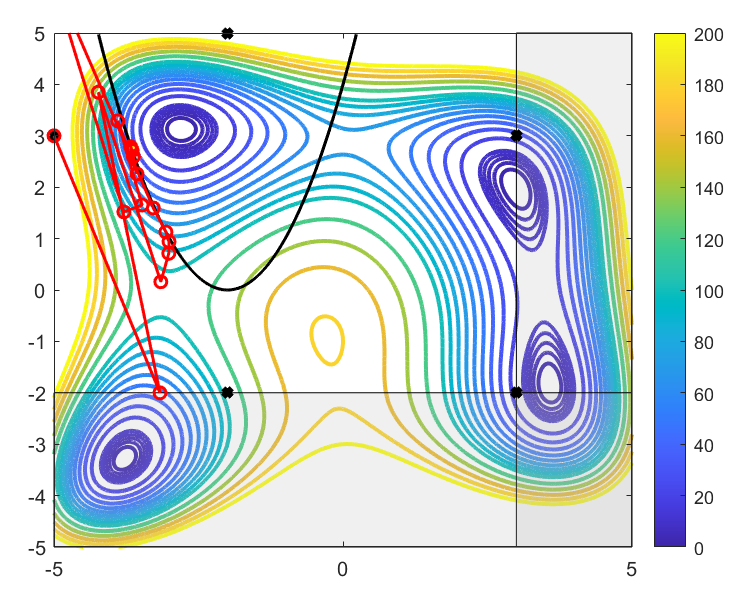
\includegraphics[scale=0.4]{figures/SQP_BFGS_LINE_A.PNG}
%\caption{fig1}
}
\quad
\subfigure[$B(-2,-2)$]{
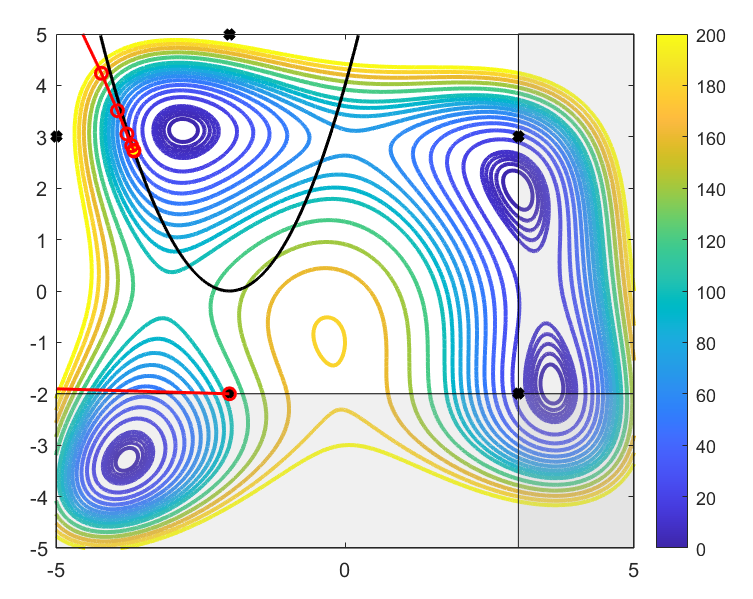
\includegraphics[scale=0.4]{figures/SQP_BFGS_LINE_B.PNG}
}
\quad
\subfigure[$C(3,3)$]{
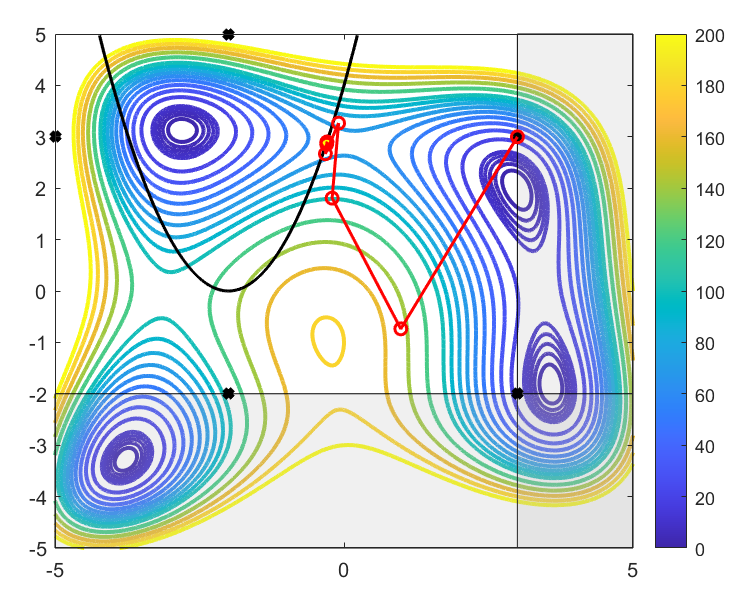
\includegraphics[scale=0.4]{figures/SQP_BFGS_LINE_C.PNG}
}
\quad
\subfigure[$D(-2,5)$]{
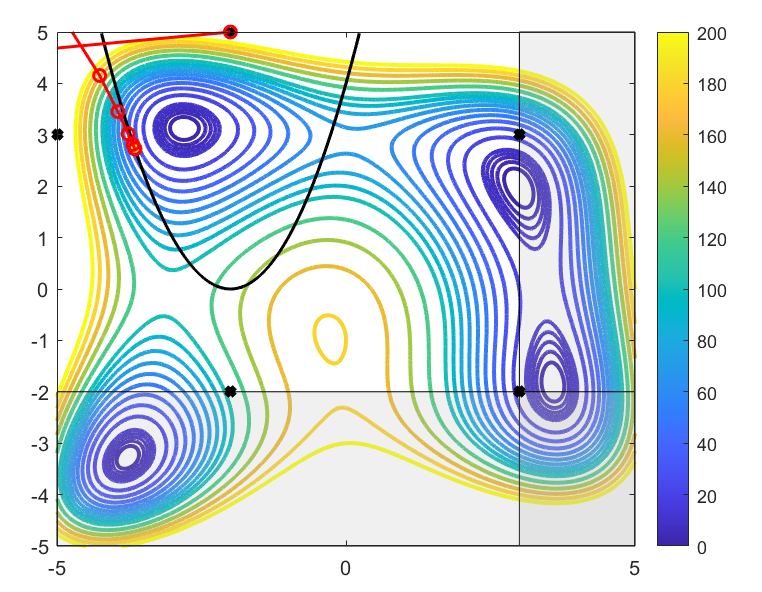
\includegraphics[scale=0.4]{figures/SQP_BFGS_LINE_D.PNG}
}
\quad
\subfigure[$E(3,-2)$]{
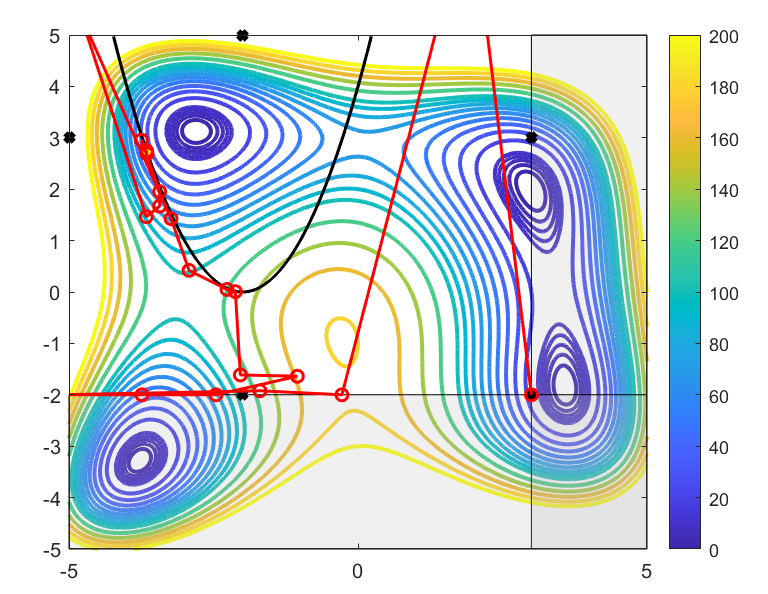
\includegraphics[scale=0.4]{figures/SQP_BFGS_LINE_E.PNG}
}
\caption{ Iterative trajectory in contour}
\end{figure}
%%%%%%%%%%%%%%%%%%%%%%%%%%%%%%%%%%%%%%%%%%%%%%%%%%%%%%%
The iteration of table is showed here separately
%%%%%%%%%%%%%%%%%%%%%%%%%%%%%%%%%%%%%%%%%%%%%%%%%%%%%%
\begin{table}[H]
\centering
\setlength{\abovecaptionskip}{0cm} 
\setlength{\belowcaptionskip}{-0.5cm}
\scriptsize
\begin{tabular}{|c|c|c|c|c|c|c|c|c|c|c|}
\hline
$x_0=A(-5,3)$&0&1&2&3&4&5&6&7&8&9\\
\hline
$x_1$&-5.0 & -3.17 & -4.23 & -3.15 & -3.01 & -3.01 & -3.06 & -3.28 & -5.09 & -3.79 \\
\hline
$x_2$&3.0 & -2.0 & 3.85 & 0.16 & 0.713 & 0.941 & 1.13 & 1.6 & 6.28 & 1.52 
\\
\hline
\end{tabular}
\begin{tabular}{|c|c|c|c|c|c|c|c|c|c|}
\hline
$x_0=A(-5,3)$&10&11&12&13&14&15&16&17&18\\
\hline
$x_1$ &3.48 & -3.9 & -3.56 & -3.63 & -3.67 & -3.65 & -3.65 & -3.65 & -3.65\\
\hline
$x_2$ & 1.65 & 3.29 & 2.26 & 2.59 & 2.79 & 2.71 & 2.74 & 2.74 & 2.74
\\
\hline

\end{tabular}
\caption{$x_0=A(-5,3)$}
\end{table}

%%%%%%%%%%%%%%%%%%%%%%%%%%%%%%%%%%%%%%%%%%%%%%%%%%%%%%%%%
\begin{table}[H]
\centering
\setlength{\abovecaptionskip}{0cm} 
\setlength{\belowcaptionskip}{-0.5cm}
\scriptsize
\begin{tabular}{|c|c|c|c|c|c|c|c|c|c|c|}
\hline
$x_0=B(-2,-2)$&0&1&2&3&4&5&6&7&8&9\\
\hline
$x_1$&-2.0 & -64.0 & -40.8 & -27.2 & -17.8 & -12.3 & -8.79 & -6.69 & -5.42 & -4.67  \\
\hline
$x_2$&-2.0 & 0 & -1.49 & 70.8 & 16.4 & 15.7 & 11.5 & 8.89 & 6.79 & 5.31   
\\
\hline
\end{tabular}

\begin{tabular}{|c|c|c|c|c|c|c|c|c|}
\hline
$x_0=B(-2,-2)$&10&11&12&13&14&15&16&17\\
\hline
$x_1$&-4.21 & -3.94 & -3.77 & -3.69 & -3.65 & -3.65 & -3.65 & -3.65  \\
\hline
$x_2$&4.24 & 3.51 & 3.06 & 2.83 & 2.72 & 2.74 & 2.74 & 2.74
\\
\hline
\end{tabular}

\caption{$x_0=B(-2,-2)$}
\end{table}
%%%%%%%%%%%%%%%%%%%%%%%%%%%%%%%%%%%%%%%%%%%%%%%%%%%%%%%%%%%%%
\begin{table}[H]
\centering
\setlength{\abovecaptionskip}{0cm} 
\setlength{\belowcaptionskip}{-0.5cm}
\scriptsize
\begin{tabular}{|c|c|c|c|c|c|c|c|c|c|c|}
\hline
$x_0=C(3,3)$&0&1&2&3&4&5&6&7&8&9\\
\hline
$x_1$&3.0 & 0.983 & -0.206 & -0.0934 & -0.322 & -0.299 & -0.294 & -0.299 & -0.298 & -0.298 \\
\hline
$x_2$&3.0 & -0.736 & 1.81 & 3.27 & 2.67 & 2.86 & 2.9 & 2.89 & 2.9 & 2.9
\\
\hline
\end{tabular}

\caption{$x_0=C(3,3)$}
\end{table}
%%%%%%%%%%%%%%%%%%%%%%%%%%%%%%%%%%%%%%%%%%%%%%%%%%%%%%%%%%%%%%%
\begin{table}[H]
\centering
\setlength{\abovecaptionskip}{0cm} 
\setlength{\belowcaptionskip}{-0.5cm}
\scriptsize
\begin{tabular}{|c|c|c|c|c|c|c|c|c|c|c|}
\hline
$x_0=D(-2,5)$&0&1&2&3&4&5&6&7&8&9\\
\hline
$x_1$&-2.0 & -50.0 & -32.1 & -21.4 & -14.1 & -9.83 & -7.22 & -5.68 & -4.79 & -4.26  \\
\hline
$x_2$&5.0 & 0 & -1.49 & 36.5 & 7.73 & 7.46 & 6.86 & 6.04 & 5.1 & 4.15
\\
\hline
\end{tabular}
\begin{tabular}{|c|c|c|c|c|c|c|c|c|c|c|c|}
\hline
$x_0=D(-2,5)$&10&11&12&13&14&15&16\\
\hline
$x_1$ &-3.95 & -3.77 & -3.69 & -3.65 & -3.65 & -3.65 & -3.65\\
\hline
$x_2$&  3.45 & 3.02 & 2.81 & 2.72 & 2.74 & 2.74 & 2.74
\\
\hline

\end{tabular}
\caption{$x_0=D(-2,5)$}
\end{table}
%%%%%%%%%%%%%%%%%%%%%%%%%%%%%%%%%%%%%%%%%%%%%%%%%%%%%%%%%%%
\begin{table}[H]
\centering
\setlength{\abovecaptionskip}{0cm} 
\setlength{\belowcaptionskip}{-0.5cm}
\scriptsize
\begin{tabular}{|c|c|c|c|c|c|c|c|c|c|c|}
\hline
$x_0=E(3,-2)$&0&1&2&3&4&5&6&7&8&9\\
\hline
$x_1$&3.0 & 1.95 & -0.278 & -1.7 & -5.15 & -3.74 & -2.46 & -1.05 & -2.04 & -2.12  \\
\hline
$x_2$&-2.0 & 7.67 & -2.0 & -1.92 & -2.0 & -2.0 & -2.0 & -1.64 & -1.61 & 0.00732 
\\
\hline
\end{tabular}
\begin{tabular}{|c|c|c|c|c|c|c|c|c|c|c|}
\hline
$x_0=E(3,-2)$&10&11&12&13&14&15&16&17&18&19\\
\hline
$x_1$ &-2.27 & -2.92 & -3.24 & -4.81 & -3.66 & -3.43 & -3.43 & -3.75 & -3.65 & -3.66\\
\hline
$x_2$&   0.05 & 0.42 & 1.43 & 5.4 & 1.46 & 1.67 & 1.95 & 2.96 & 2.69 & 2.75
\\
\hline

\end{tabular}
\begin{tabular}{|c|c|c|c|}
\hline
$x_0=E(3,-2)$&20&21&22\\
\hline
$x_1$ &-3.65 & -3.65 & -3.65\\
\hline
$x_2$&   2.74 & 2.74 & 2.74
\\
\hline

\end{tabular}
\caption{$x_0=E(3,-2)$}
\end{table}

It can be seen that starting points $A$, $B$,$D$, and $E$ have reached the correct minimum points, but starting points $C$ reached a sub-minimum point. The success rate of SQP with BFGS and line search is higher than the previous algorithm(without line search), and the number of iterations is also reduced compared to the previous algorithm\\

First analyze from the contours with starting points $B$ and $D$. These two points in the previous algorithm(without line search) can only find the sub-minimum point because the step size of the sub-problem solution is too large, but after adding the line search algorithm, it is found that the amplitude of the step size did not change too much, so the minimum point was successfully found. Similarly, the points $C$ and $E$ mentioned earlier accidentally crossed the area where the maximum point was found because of the large step size, but after adding the line search, although the step size of $E$ point is still too large , the step size of point $C$ is obviously suppressed, and the sub-minimum point is found in the right half of the equality constraint curve.

%%%%%%%%%%%%%%%%%%%%%%%%%%%%%%%%%%%%%%%%%%
%%%%%%%%%%%%%%%%%%%%%%%%%%%%%%%%%%%%%%%%%%%
%%%%%%%%%%%%%%%%%%%%%%%%%%%%%%%%%%%%%%%%%%
%%%%%%%%%%%%%%%%%%%%%%%%%%%%%%%%%%%%%%%%%%%
%%%%%%%%%%%%%%%%%%%%%%%%%%%%%%%%%%%%%%%%%%
%%%%%%%%%%%%%%%%%%%%%%%%%%%%%%%%%%%%%%%%%%%
\newpage
\subsection{\bfseries Trust Region based SQP algorithm}
\begin{shaded}
{Question:Explain, discuss, and implement a Trust Region based SQP algorithm for this
problem. Make a table with the iteration sequence. Make a table with
relevant statistics (function calls etc). Plot the iteration sequence in a contour
plot. Discuss the results}
\end{shaded}
In the trust region method, the parameter $\Delta _k$ is used to control the quality of the steps as the size of the trust region. The simplest way to formulate a trust-region SQP method is to add a trust-region constraint to subproblem

$$\begin{aligned}
\min _{\Delta x \in \mathbb{R}^{n}} \qquad & \frac{1}{2} \Delta x^{\prime}\left[\nabla_{x x}^{2} L\left(x_{k}, \mu_{k},\lambda_{k}\right)\right] \Delta x+\left[\nabla_{x} L\left(x_{k}, \mu_{k},\lambda_{k}\right)\right]^{\prime} \Delta x \\
\text {s.t.} \qquad & \nabla g\left(x_{k}\right)^{\prime} \Delta x=-g\left(x_{k}\right)\\
& \nabla h\left(x_{k}\right)^{\prime} \Delta x\ge -h\left(x_{k}\right)\\
& \left\| p\right \|\le \Delta_k
\end{aligned}\eqno{(5.37)}$$

However, even if the constraints are compatible, this problem may not always have a solution because of the trust-region constraint. Here, the S$l1$QP is introduced. In this approach the linearized constraints are moved into the objective of the quadratic program, in the form of an $l1$ penalty term, to obtain the following subproblem by introducing
slack variables $v4$, $w$, $t$:
\begin{align*}
\min _{p, v, w, t} \quad &f_{k}+\nabla f_{k}^{T} p+\frac{1}{2} p^{T} \nabla_{x x}^{2} \mathcal{L}_{k} p+\mu \sum_{i \in \mathcal{E}}\left(v_{i}+w_{i}\right)+\mu \sum_{i \in \mathcal{I}} t_{i}\tag{5.38}\\
s.t.\quad & \nabla g_{i}\left(x_{k}\right)^{T} p+g_{i}\left(x_{k}\right)=v_{i}-w_{i}\\
&\nabla h_{i}\left(x_{k}\right)^{T} p+h_{i}\left(x_{k}\right) \geq-t_{i}\\
&v, w, t \geq 0\\
&\|p\|_{\infty} \leq \Delta_{k}
\end{align*}

This formulation is simply a linearization of the elastic-mode formulation with the
addition of a trust-region constraint.
The constraints of this problem are always consistent. Since the trust region has been
defined using the $l \infty$ norm, is a smooth quadratic program that can be solved
by means of a quadratic programming algorithm.\\
\newpage
After computing the step $p_k$, the ratio $\rho_k$ is determined via

$$\rho_{k}=\frac{\operatorname{ared}_{k}}{\operatorname{pred}_{k}}=\frac{\phi_{1}\left(x_{k}, \mu\right)-\phi_{1}\left(x_{k}+p_{k}, \mu\right)}{q_{\mu}(0)-q_{\mu}\left(p_{k}\right)}\eqno{(5.39)}$$

Use the merit function $\phi1$ and defining $q_{\mu}$ by

$$q_{\mu}(p)=f_{k}+\nabla f_{k}^{\prime} p+\frac{\sigma}{2} p^{\prime} \nabla_{x x}^{2} \mathcal{L}_{k} p+\mu m_{k}(p)\eqno{(5.40)}$$
Where
$$m(p)=\left\|g(x_k)+\nabla g(x_k)p_k\right\|_1+\left\|h(x_k)+\nabla h(x_k)p_k\right\|_1\eqno{(5.41)}$$

Then the most important step is to choose a suitable $\mu$ at each iterates, because the $\mu$ plays an important role in the efficiency of this method. The step $p_k$ directly depends on the value of $\mu$. Values of $\mu$ that are too small can lead the algorithm away from the solution, while excessively large values can result in slow progress. A penalty update and step computation algorithm is stated here


\begin{algorithm}[H]
	\caption{ Penalty Update}
	\begin{algorithmic}[1]
	    \STATE Given $x_k,\mu_{k-1}>0$,$\delta_k>0$,and parameters $\eta_1,\eta_2 \in (0,1)$\\
		\IF{($m_k(p(\mu_{k-1}))$)}\\
		\STATE Set $\mu_k=\mu_{k-1}$\\
        \ELSE\\
		\STATE Compute the $p_{\infty}$\\
		\IF{($m_k(p_{\infty})$)}\\
		\STATE Find $\mu{k}>\mu_{k-1}$ such that $m_k(p(\mu_{k}))=0$\\
		\ELSE\\
		\STATE Find $\mu{k}>\mu_{k-1}$ such that$m_k(0)-m_k(p(\mu_{k}))\ge \eta_1\left[m_k(0)-m_k(p(\infty)\right]$
		\ENDIF\\
		\ENDIF\\
		\STATE increas $\mu_k$ if necessary to satisfy$q_{\mu_k}(0)-q_{\mu_k}(p(\mu_k))\ge \eta_2\mu_k\left[m_k(0)-m_k(p(\mu_{k}))\right]$
    \end{algorithmic}
\end{algorithm}

The step is accepted or rejected
according to standard trust-region rules, as implemented in pseudo-code\\
\newpage
{\setmainfont{Times New Roman}\bfseries Pseudo-code}
\begin{algorithm}[H]
	\caption{ Trust Region based SQP algorithm}
	\begin{algorithmic}[1]
	    \STATE Given a starting point($x_0,\mu_0,\lambda_0$), set $k=0$. Choose $\eta \in (0,1), \tau \in (0,0.5)$\\
		\STATE Evaluate $f_0,\nabla f_0,g_0,\nabla g_0,h_0,\nabla h_0$\\
		\STATE Choose an initial $n \times n$ symmetric positive definite Hessian approximation $B_0$, always an Identity matrix\\
        \WHILE {(not converged)}\\
		\STATE Compute the $p_k$($\Delta x_k$),$\mu_{k+1}$ and $\lambda_{k+1}$by solving the sub-quadratic-problem\\
		\STATE Set $p_{\lambda}=\lambda_{k+1}-\lambda_{k}$\\
		\STATE Compute $\mu$ with the penalty update algorithm stated above\\
		\STATE Compute $\rho_k=ared_k/pred_k$\\
		\IF{($\rho_k>\eta$)}\\
		\STATE Set $x_{k+1}=x_k+p_k$\\
		\STATE Choose $\Delta_{K+1}$ to satisfy $\Delta_{K+1}\ge \Delta_{K}$\\
		\ELSE\\
		\STATE Set $x_{k+1}=x_k$\\
		\STATE Choose $\Delta_{K+1}$ to satisfy $\Delta_{K+1}\le \gamma \|p_k\|$\\
		\ENDIF\\
		\STATE Compute $\nabla_{x}L\left(x_{k}, \mu_{k+1},\lambda_{k+1}\right)=\nabla f(x_k)-\nabla g(x_k)\mu_{k+1}-\nabla h(x_k)\lambda_{k+1}$\\
		\STATE Evaluate $f_{k+1},\nabla f_{k+1},g_{k+1},\nabla g_{k+1},h_{k+1},\nabla h_{k+1}$\\
		\STATE Compute $\nabla_{x}L\left(x_{k+1}, \mu_{k+1},\lambda_{k+1}\right)=\nabla f(x_{k+1})-\nabla g(x_{k+1})\mu_{k+1}-\nabla h(x_{k+1})\lambda_{k+1}$\\
		\STATE Compute the $s_k$ and $y_k$\\
		\STATE Update the Hessian matrix by the modified BFGS procedure\\
		\STATE $k=k+1$\\
		\ENDWHILE
    \end{algorithmic}
\end{algorithm}



Next the specific Matlab code of implementation is showed. The function "Hg_f" which calculate the gradients and hessian of object-function and itself, the "Hg_ceq" which calculate the gradients and hessian of equality constraints and itself, the "Hg_ciq" which calculate the gradients and hessian of equality constraints and itself, the "Qpsolver_Sqp" which solve the sub-problem of SQP algorithm are stated in appendix \ref{6.5.4}, \ref{6.5.5}, \ref{6.5.6} and \ref{6.5.7}. Only the main program is showed here

{\setmainfont{Courier New Bold} \scriptsize         
\begin{lstlisting}
function [x,output]=Sqp_Bfgs_trust(x0,lam_eq0,lam_ineq0)
% Sqp_Bfgs_trust   SQP algorithm with damped BFGS and line search
%
%          min  f(x)
%           x
%          s.t. ceq(x)=0  (Lagrange multiplier lam_eq)    
%               ciq(x)>=0  (Lagrange multiplier lam_ineq)  
% Syntax: [x,output]=Sqp_Bfgs_trust(x0,lam_eq0,lam_ineq0)
%         output.fval: minimum value
%         output.dL: convergence of delta_L
%         output.ceq: convergence of ceq
%         output.Xarray=Xarray: Iteration trajectory  
epsilon=1e-6;
ro=0.99;
gamma=0.9;
eta=0.2;
eta2=0.2;
eta3=0.5;
deltak=0.9;

deltaAarray=[];
deltaAarray=[deltaAarray deltak];
mu=30;
Xarray=[];
normdLarray=[];
normceqarray=[];
Xarray=[Xarray x0];

nx=size(x0,1);
Bk=eye(nx);

[f,df,~]=Hg_f(x0);
[ceq,dceq,~]=Hg_ceq(x0);
[ciq,dciq,~]=Hg_ciq(x0);

xk=x0;
lam_eqk=lam_eq0;
lam_ineqk=lam_ineq0;
iteration=0;
iteration_max=80;
iter_line_max=30;
while(iteration<iteration_max)
    %Solve the subproblem(QP)
    %Linearization of the elastic-mode formulation
    
    H_L1=[Bk zeros(2,2) zeros(2,2);zeros(4,6)];
    df_L1=[df;mu;mu;mu;mu];
    dciq_L1=[dciq' [1 0 0 0;0 1 0 0];zeros(4,2) eye(4);...
       [1 0 0 0 0 0];[0 1 0 0 0 0];[-1 0 0 0 0 0];[0 -1 0 0 0 0]];
    ciq_L1=[-ciq;zeros(4,1);-deltak;-deltak;-deltak;-deltak];
    dceq_L1=[dceq' 0 0 -1 1];
    ceq_L1=[-ceq];
    [p_all,~,~,~,lamk] = quadprog(H_L1,df_L1,-dciq_L1,-ciq_L1,dceq_L1,ceq_L1);
    p=p_all(1:2);
    lamineq=lamk.ineqlin(1:2); 
    
    lameq=lamk.eqlin;
    lam_eqk_hat=-lameq;
    lam_ineqk_hat=-lamineq;
    lam_eqk=lam_eqk_hat;
    lam_ineqk=lam_ineqk_hat;
    
    %evaluate the gradient
    [f_new,~,~]=Hg_f(xk+p);
    [ceq_new,~,~]=Hg_ceq(xk+p);
    [ciq_new,~,~]=Hg_ciq(xk+p);
    
   
    mp_eq=norm((ceq+dceq'*p),1);
    mp_ineq=norm(min(0,(ciq+dciq'*p)),1);
    mp_k=mp_eq+mp_ineq;
    %Penalty update and step computation
    if mp_k==0
        mu=mu;
    else
        p_norm=norm(p,"Inf");
        mp_eq_inf=norm((ceq+dceq'*p),1);
        mp_ineq_inf=norm(min(0,(ciq+dciq'*p)),1);
        mp_k_inf=mp_eq+mp_ineq;
        if mp_k_inf==0
            mu=mu*(1+eta2);
        else
        if norm(ceq,1)+norm(min(0,ciq),1)-mp_k>=eta3*(norm(ceq,1)+norm(min(0,ciq),1)-mp_k_inf)
            mu=mu;
        else
            mu=mu*(1+eta2);
        end
        end
    end
    %calculate the ratio
    qmu_p=f+df'*p+0.5*p'*Bk*p+mu*mp_eq+mu*mp_ineq;
    qmu_zero=f+mu*norm((ceq),1)+mu*norm(min(0,ciq),1);
    predk=qmu_zero-qmu_p;
   
    phi1=f+mu*norm(ceq,1)+mu*norm(min(0,ciq),1);
    phi1_new=f_new+mu*norm(ceq_new,1)+mu*norm(min(0,ciq_new),1);
    aredk=phi1-phi1_new;
    rok=aredk/predk;
    %judge the step is accepted or rejected
    if rok>eta
        xk=xk+p;
        deltak=1.5*deltak;
    else
        deltak=gamma*norm(p,"Inf");
    end
   
    %Calculate dL(k) with x(k) and lameq(k+1),lamineq(k+1)
    Lk=df-dceq.*lam_eqk-dciq*lam_ineqk;
    %Re-evaluate
    [f,df,~]=Hg_f(xk);
    [ceq,dceq,~]=Hg_ceq(xk);
    [ciq,dciq,~]=Hg_ciq(xk);
    %Calculate L(k+1) with x(k+1) and lam(k+1)
    Lk2=df-dceq.*lam_eqk-dciq*lam_ineqk;
    %Damped BFGS update
    pk=p;
    qk=Lk2-Lk;
    
    judge=(pk'*qk>=0.2*pk'*(Bk*pk));
    thetak=judge.*1+(~judge).*((0.8*pk'*(Bk*pk))/(pk'*(Bk*pk)-pk'*qk));
    rk=thetak*qk+(1-thetak)*(Bk*pk);
    Bk=Bk-((Bk*pk)*(pk'*Bk))/(pk'*(Bk*pk))+(rk*rk')/(pk'*rk);
    %Check teh convergence
    if ((norm(Lk2,"inf")<epsilon)&&(norm(ceq,"inf")<epsilon)&&(max(abs(ciq)) + epsilon >= 0)...
       &&(min(lam_ineqk) + epsilon >= 0))
        break;
    end
    iteration=iteration+1;
    Xarray=[Xarray xk];
    normdLarray=[normdLarray norm(Lk2,"inf")];
    normceqarray=[normceqarray norm(ceq,"inf")];
    deltaAarray=[deltaAarray deltak];
end
[fval,~,~]=Hg_f(xk);
x=xk;
output.fval=fval;
output.xarray=Xarray;
output.dL=normdLarray;
output.ceq=normceqarray;
output.iteration=iteration;
output.delta=deltaAarray;
end
\end{lstlisting}}
%%%%%%%%%%%%%%%%%%%%%%%%%%%%%%%%%%%%%%%%%%%%%%%%%%%%%%%%
The algorithm will be tested with the same initial
points as in the section 5.5. Please see the test code in Appendix \ref{6.5.10}. Iterative trajectory of starting points $A$, $B$, $C$, $D$ and $E$ in the contour is showed 
\begin{figure}[H]
\centering
\subfigure[$A(-5,3)$]{
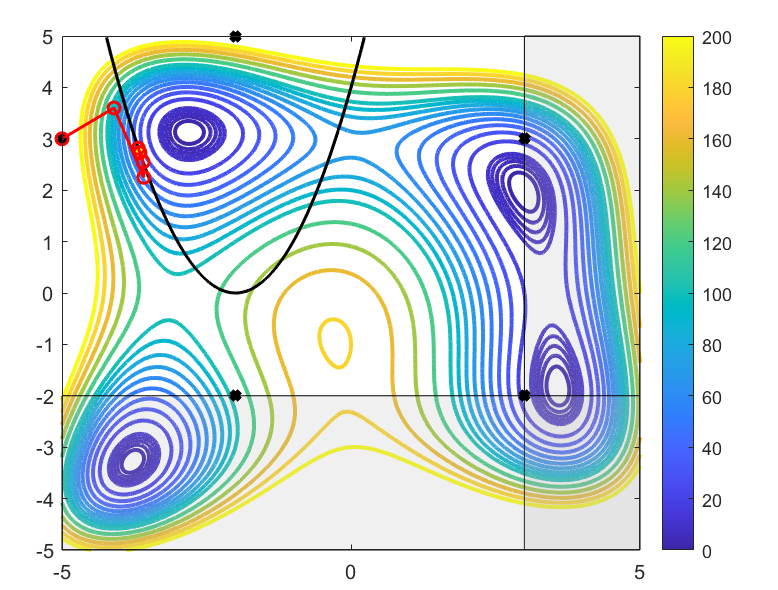
\includegraphics[scale=0.4]{figures/SQP_BFGS_TRUST_A.PNG}
%\caption{fig1}
}
\quad
\subfigure[$B(-2,-2)$]{
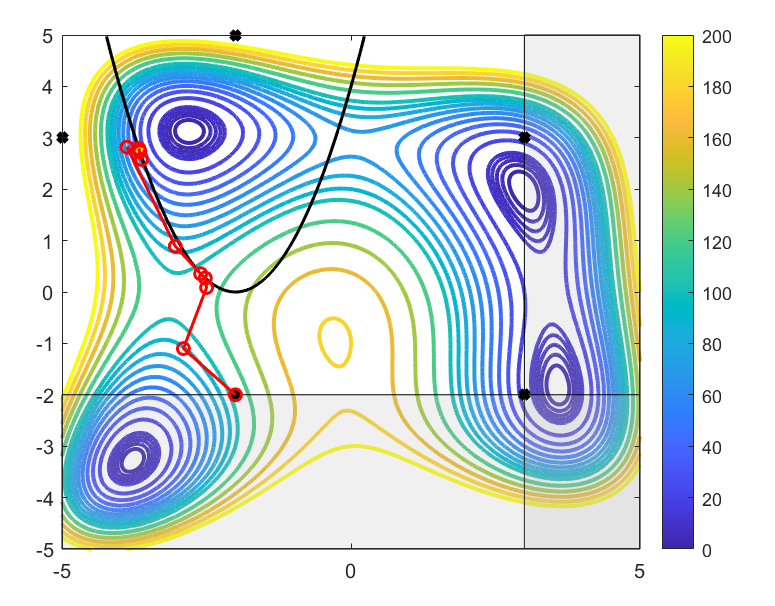
\includegraphics[scale=0.4]{figures/SQP_BFGS_TRUST_B.PNG}
}
\quad
\subfigure[$C(3,3)$]{
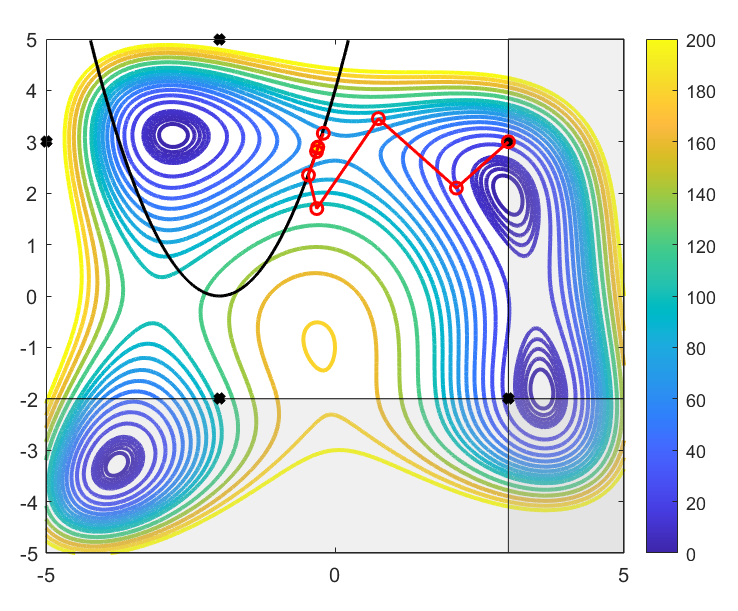
\includegraphics[scale=0.4]{figures/SQP_BFGS_TRUST_C.PNG}
}
\quad
\subfigure[$D(-2,5)$]{
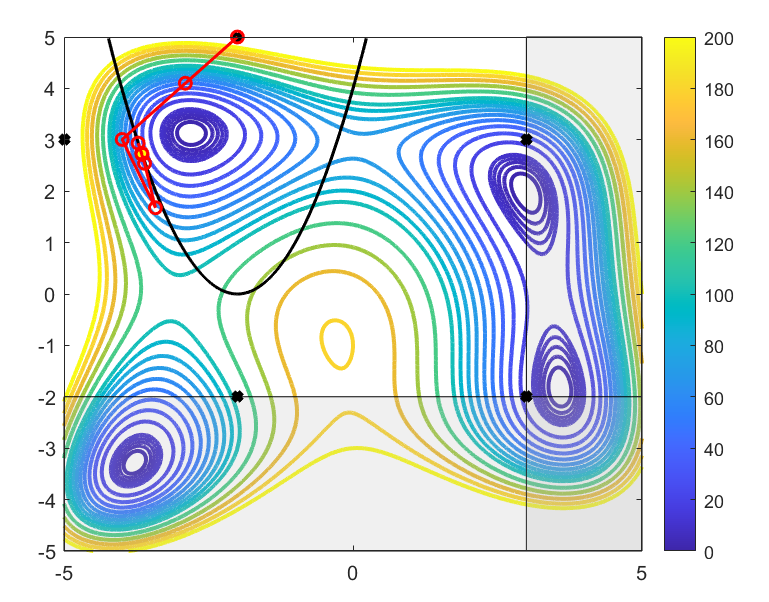
\includegraphics[scale=0.4]{figures/SQP_BFGS_TRUST_D.PNG}
}
\quad
\subfigure[$E(3,-2)$]{
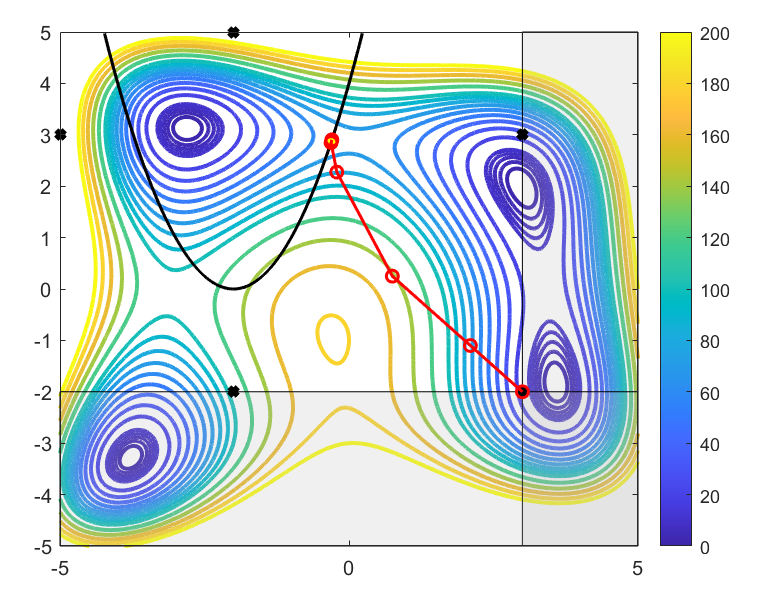
\includegraphics[scale=0.4]{figures/SQP_BFGS_TRUST_E.PNG}
}
\caption{ Iterative trajectory in contour}
\end{figure}

%%%%%%%%%%%%%%%%%%%%%%%%%%%%%%%%%%%%%%%%%%%%%%%%%%%%%%%
The iteration of table is showed here separately
%%%%%%%%%%%%%%%%%%%%%%%%%%%%%%%%%%%%%%%%%%%%%%%%%%%%%%
\begin{table}[H]
\centering
\setlength{\abovecaptionskip}{0cm} 
\setlength{\belowcaptionskip}{-0.5cm} 
\scriptsize
\begin{tabular}{|c|c|c|c|c|c|c|c|c|}
\hline
$x_0=A(-5,3)$&0&1&2&3&4&5&6&7\\
\hline
$x_1$&-5.0 & -4.1 & -3.59 & -3.6 & -3.68 & -3.65 & -3.65 & -3.65\\
\hline
$x_2$&3.0 & 3.6 & 2.25 & 2.55 & 2.82 & 2.73 & 2.74 & 2.74
\\
\hline
\end{tabular}
\caption{$x_0=A(-5,3)$}
\end{table}

%%%%%%%%%%%%%%%%%%%%%%%%%%%%%%%%%%%%%%%%%%%%%%%%%%%%%%%%%
\begin{table}[H]
\centering
\setlength{\abovecaptionskip}{0cm} 
\setlength{\belowcaptionskip}{-0.5cm} 
\scriptsize
\begin{tabular}{|c|c|c|c|c|c|c|c|c|c|c|}
\hline
$x_0=B(-2,-2)$&0&1&2&3&4&5&6&7&8&9\\
\hline
$x_1$&-2.0 & -2.9 & -2.5 & -2.52 & -2.6 & -3.04 & -3.04 & -3.04 & -3.04 & -3.04 \\
\hline
$x_2$&-2.0 & -1.1 & 0.0876 & 0.271 & 0.355 & 0.888 & 0.888 & 0.888 & 0.888 & 0.888 
\\
\hline
\end{tabular}

\begin{tabular}{|c|c|c|c|c|c|c|c|c|c|c|}
\hline
$x_0=B(-2,-2)$&10&11&12&13&14&15&16&17&18&19\\
\hline
$x_1$&-3.04 & -3.04 & -3.04 & -3.04 & -3.04 & -3.04 & -3.04 & -3.04 & -3.88 & -3.63  \\
\hline
$x_2$&0.888 & 0.888 & 0.888 & 0.888 & 0.888 & 0.888 & 0.888 & 0.888 & 2.82 & 2.58
\\
\hline
\end{tabular}
\begin{tabular}{|c|c|c|c|c|}
\hline
$x_0=B(-2,-2)$&20&21&22&23\\
\hline
$x_1$ &-3.67 & -3.65 & -3.65 & -3.65\\
\hline
$x_2$&  2.79 & 2.73 & 2.74 & 2.74\\
\hline

\end{tabular}
\caption{$x_0=B(-2,-2)$}
\end{table}
%%%%%%%%%%%%%%%%%%%%%%%%%%%%%%%%%%%%%%%%%%%%%%%%%%%%%%%%%%%%%
\begin{table}[H]
\centering
\setlength{\abovecaptionskip}{0cm} 
\setlength{\belowcaptionskip}{-0.5cm} 
\scriptsize
\begin{tabular}{|c|c|c|c|c|c|c|c|c|c|c|}
\hline
$x_0=C(3,3)$&0&1&2&3&4&5&6&7&8&9\\
\hline
$x_1$&3.0 & 2.1 & 0.75 & -0.316 & -0.46 & -0.202 & -0.32 & -0.301 & -0.298 & -0.298 \\
\hline
$x_2$&3.0 & 2.1 & 3.45 & 1.7 & 2.35 & 3.17 & 2.81 & 2.89 & 2.9 & 2.9
\\
\hline
\end{tabular}

\caption{$x_0=C(3,3)$}
\end{table}
%%%%%%%%%%%%%%%%%%%%%%%%%%%%%%%%%%%%%%%%%%%%%%%%%%%%%%%%%%%%%%%
\begin{table}[H]
\centering
\setlength{\abovecaptionskip}{0cm} 
\setlength{\belowcaptionskip}{-0.5cm} 
\scriptsize
\begin{tabular}{|c|c|c|c|c|c|c|c|c|c|c|}
\hline
$x_0=D(-2,5)$&0&1&2&3&4&5&6&7&8&9\\
\hline
$x_1$&-2.0 & -2.9 & -2.9 & -2.9 & -3.99 & -3.99 & -3.99 & -3.42 & -3.61 & -3.61  \\
\hline
$x_2$&5.0 & 4.1 & 4.1 & 4.1 & 3.01 & 3.01 & 3.01 & 1.68 & 2.54 & 2.54
\\
\hline
\end{tabular}
\begin{tabular}{|c|c|c|c|c|c|}
\hline
$x_0=D(-2,5)$&10&11&12&13&14\\
\hline
$x_1$ &-3.72 & -3.65 & -3.65 & -3.65 & -3.65\\
\hline
$x_2$& 2.94 & 2.72 & 2.74 & 2.74 & 2.74
\\
\hline

\end{tabular}
\caption{$x_0=D(-2,5)$}
\end{table}
%%%%%%%%%%%%%%%%%%%%%%%%%%%%%%%%%%%%%%%%%%%%%%%%%%%%%%%%%%%
\begin{table}[H]
\centering
\setlength{\abovecaptionskip}{0cm} 
\setlength{\belowcaptionskip}{-0.5cm} 
\scriptsize
\begin{tabular}{|c|c|c|c|c|c|c|c|c|}
\hline
$x_0=E(3,-2)$&0&1&2&3&4&5&6&7\\
\hline
$x_1$&3.0 & 2.1 & 0.75 & -0.211 & -0.31 & -0.296 & -0.298 & -0.298 \\
\hline
$x_2$&-2.0 & -1.1 & 0.25 & 2.27 & 2.85 & 2.9 & 2.9 & 2.9
\\
\hline
\end{tabular}

\caption{$x_0=E(3,-2)$}
\end{table}
It can be seen that starting points $A$, $B$, and $D$ have reached the correct minimum points, but starting points $C$ and $E$ reached a sub-minimum point, which has the same result as one solved by fmincon.\\
From the contours of $A$, $B$, and $D$ starting points that successfully reach the minimum point, the step size of each iteration is adjusted appropriately, and the minimum point can be reached with a small number of iterations. The effect is obviously better than the line search method. At the same time, from the contours of $C$ and $E$ starting points that reach the sub-minimum point. Because the step size is appropriately limited, there is no large jump in iteration process of $C$ and $E$ as before, skipping the area where the maximum value is, and accidentally reaching the left half part of the equality constraint curve and finds the minimum point, but iterates normally to the right half part of the equality constraint curve and finds the sub-minimum point.
Through the comparison of these three methods(SQP with BFGS, SQP with BFGS and line search, SQP based on trust region), it is found that the trust region based method adjusts the step size more accurately, can be more stable, and obtain better results.
%%%%%%%%%%%%%%%%%%%%%%%%%%%%%%%%%%%%%%%%%%
%%%%%%%%%%%%%%%%%%%%%%%%%%%%%%%%%%%%%%%%%%%
%%%%%%%%%%%%%%%%%%%%%%%%%%%%%%%%%%%%%%%%%%
%%%%%%%%%%%%%%%%%%%%%%%%%%%%%%%%%%%%%%%%%%%
%%%%%%%%%%%%%%%%%%%%%%%%%%%%%%%%%%%%%%%%%%
%%%%%%%%%%%%%%%%%%%%%%%%%%%%%%%%%%%%%%%%%%%
\subsection{\bfseries Primal-Dual Interior Point Algorithms for NLP}
\begin{shaded}
{Question:Explain, discuss, and implement an interior-point algorithm for this problem.
Make a table with the iteration sequence. Make a table with relevant statistics
(function calls etc). Plot the iteration sequence in a contour plot. Discuss the
results}
\end{shaded}
First, the nonlinear problem can be written as follows by introducing the slack variables

$$\begin{aligned}
\min _{x,s} \qquad & f(x) \\
\text {s.t.} \qquad & g(x)=0\\
& h(x)-s=0\\
& s\ge 0
\end{aligned}\eqno{(5.42)}$$

Then the KKT condition can be expressed as
\begin{align*}
&\nabla_{x} L(x, y, z)=\nabla f(x)-\nabla g(x) y-\nabla h(x) z=0 \tag{5.43}\\
&g(x)=0 \tag{5.44}\\
&h(x)-s=0 \tag{5.45}\\
&S z=0 \tag{5.46}\\
&s \geq 0 \quad z \geq 0 \tag{5.47}
\end{align*}
In the interior point algorithms a perturbed KKT system is solved

$$S z=0 \Leftrightarrow Sz-\tau e=0\eqno{(5.48)}$$

Then apply the Newton's method and obtain the primal-dual system

$$\left[\begin{array}{cccc}
\nabla_{x x}^{2} L(x, y, z) & 0 & -\nabla g(x) & -\nabla h(x) \\
0 & Z & 0 & S \\
\nabla g(x)^{\prime} & 0 & 0 & 0 \\
\nabla h(x)^{\prime} & -I & 0 & 0
\end{array}\right]\left[\begin{array}{c}
p_{x} \\
p_{s} \\
p_{y} \\
p_{z}
\end{array}\right]=-\left[\begin{array}{c}
\nabla_{x} L(x, y, z) \\
S z-\tau e \\
g(x) \\
h(x)-s
\end{array}\right]\eqno{(5.49)}$$
which is equivalent to the symmetric system

$$\left[\begin{array}{cccc}
\nabla_{x x}^{2} L(x, y, z) & 0 & \nabla g(x) & \nabla h(x) \\
0 & \Sigma & 0 & -I \\
\nabla g(x)^{\prime} & 0 & 0 & 0 \\
\nabla h(x)^{\prime} & -I & 0 & 0
\end{array}\right]\left[\begin{array}{c}
p_{x} \\
p_{s} \\
-p_{y} \\
-p_{z}
\end{array}\right]=-\left[\begin{array}{c}
\nabla_{x} L(x, y, z) \\
z-\tau S^{-1} e \\
g(x) \\
h(x)-s
\end{array}\right]\eqno{(5.50)}$$
Where
$$\Sigma =S^{-1}Z\eqno{(5.51)}$$
Compute the step length 

$$\begin{array}{l}
\alpha_{s}=\max \left\{\alpha \in(0,1]: s+\alpha p_{s} \geq \eta s\right\}\eqno{(5.52)} \\
\alpha_{z}=\max \left\{\alpha \in(0,1]: z+\alpha p_{z} \geq \eta z\right\}\eqno{(5.53)}
\end{array}$$

Then update the new iterate
\begin{align*}
    x_{k+1}&=x_k+ \alpha_sp_x \tag{5.54}\\
    s_{k+1}&=s_k+ \alpha_sp_s\tag{5.55}\\
    y_{k+1}&=y_k+ \alpha_zp_y\tag{5.56}\\
    z_{k+1}&=z_k+ \alpha_zp_z\tag{5.57}
\end{align*}
About the check of convergence, the error measure is defined

$$E(x, s, y, z ; \tau)=\|F(x, s, y, z ; \tau)\|\eqno{(5.58)}$$
Where
$$\begin{aligned}
&F(x, s, y, z ; \tau)=\left[\begin{array}{c}
\nabla_{x} L(x, y, z) \\
S z-\tau e \\
g(x) \\
h(x)-s
\end{array}\right]=\left[\begin{array}{l}
0 \\
0 \\
0 \\
0
\end{array}\right]=0\\
&(s, z) \geq 0
\end{aligned}\eqno{(5.59)}$$
\newpage
{\setmainfont{Times New Roman}\bfseries Pseudo-code}
\begin{algorithm}[H]
	\caption{Primal-Dual Interior Point Algorithms for NLP}
	\begin{algorithmic}[1]
	    \STATE Choose $x_0$,$s_0>0$. Compute initial values for $y_0$, $z_0$\\
		\STATE Select $\tau_0$, $\eta=0.005$,$\rho \in (0,1)$, $k=0$\\
		\WHILE {($E(x_k,s_k,y_k,z_k,0)>\epsilon$)}\\
		\WHILE {($E(x_k,s_k,y_k,z_k,\tau_k)>\tau_k$)}\\
		\STATE Solve the primal-dual system to obtain the search direction $p_x$, $p_s$, $p_y$, $p_z$.\\
		\STATE Compute the step length $\alpha_s^{max}$, $\alpha_z^{max}$\\
		\STATE Update the iterate $x_{k+1}$, $s_{k+1}$, $y_{k+1}$, $z_{k+1}$, $k=k+1$\\
		\ENDWHILE\\
		\STATE Choose $\tau_k \in (0,\rho  \tau_k)$\\
		\ENDWHILE
    \end{algorithmic}
\end{algorithm}
Next the specific Matlab code of implementation is showed. The function "Hg_f" which calculate the gradients and hessian of object-function and itself, the "Hg_ceq" which calculate the gradients and hessian of equality constraints and itself, the "Hg_ciq" which calculate the gradients and hessian of equality constraints and itself are stated in Appendix \ref{6.5.4}, \ref{6.5.5} and \ref{6.5.6}. Only the main program is showed here

{\setmainfont{Courier New Bold} \scriptsize         
\begin{lstlisting}
function [x,output]=ipNLP(x0,y0,z0,s0)
% ipNLP   Primal-Dual Interior Point Algorithms for NLP
%
%          min  f(x)
%           x
%          s.t. ceq(x)=0  (Lagrange multiplier y)    
%               ciq(x)-s=0  (Lagrange multiplier z)
%               s>=0
%          rdL=df-dceq*y-dciq*z;
%          rsz=S*z-tau*e;
%          rceq=ceq;
%          rciq=ciq-s;
% Syntax: [x,output]=ipNLP(x0,y0,z0,s0)
%         output.fval: minimum value
%         output.Xarray=Xarray: Iteration trajectory  
epsilon=1.0e-5;
tau0=0.8;
eta=0.005;
ro=0.5;
Xarray=[];
Xarray=[Xarray x0];

nx=size(x0,1);
neq=size(y0,1);
niq=size(z0,1);
e=ones(niq,1);
%evaluate the gradient and hessian
[f,df,d2f]=Hg_f(x0);
[ceq,dceq,d2ceq]=Hg_ceq(x0);
[ciq,dciq,d2ciq]=Hg_ciq(x0);

xk=x0;
yk=y0;
Z0=diag(z0);
S0=diag(s0);
Zk=Z0;
Sk=S0;
tauk=tau0;
iteration=0;
iteration_out=0;
iteration_max=700;
iteration_max_out=700;
while(iteration_out<iteration_max_out)
    %convergence judge
    
    rdL=df-dceq*yk-dciq*diag(Zk);
    rsz=Sk*diag(Zk)-0*e;
    rceq=ceq;
    rciq=ciq-diag(Sk);
    Error=max([norm(rdL,1),norm(rsz,1),norm(rceq,1),norm(rciq,1)]);
    if Error<epsilon
        break;
    end
    while(iteration<iteration_max)
        %solve the subproblem
        [f,df,d2f]=Hg_f(xk);
        [ceq,dceq,d2ceq]=Hg_ceq(xk);
        [ciq,dciq,d2ciq]=Hg_ciq(xk);
        sk=diag(Sk);
        zk=diag(Zk);
        sumeq=0;
        sumiq=0;
        for i=1:length(yk)
            sumeq=sumeq+yk(i)*d2ceq(:,:,i);
        end
        for i=1:length(zk)
            sumiq=sumiq+zk(i)*d2ciq(:,:,i);
        end
        ddL=d2f-sumeq-sumiq;
        sumk=inv(Sk)*Zk;
        KKT_A=[ddL,zeros(nx,niq),dceq,dciq;zeros(niq,nx),sumk,zeros(niq,neq),-eye(niq);...
           dceq',zeros(neq,niq),zeros(neq,neq),zeros(neq,niq);dciq',-eye(niq),zeros(niq,neq),...
           zeros(niq,niq)];
        rdL=df-dceq*yk-dciq*zk;
        rsz=zk-tauk.*inv(Sk)*e;
        rceq=ceq;
        rciq=ciq-sk;
        KKT_b=-[rdL;rsz;rceq;rciq];
        [L,D,p]=ldl(KKT_A,'vector');
        p_all=zeros(size(KKT_b,1),1);
        p_all(p)=L'\(D\(L\KKT_b(p)));
        px=p_all(1:nx);
        ps=p_all(nx+1:nx+niq);
        py=-p_all(nx+niq+1:nx+niq+neq);
        pz=-p_all(nx+niq+neq+1:end);
        %compute the step length
        alpha_tmp_s=(eta.*sk-sk)./ps;
        alpha_s=min([1;alpha_tmp_s(ps<0)]);
        alpha_tmp_z=(eta.*zk-zk)./pz;
        alpha_z=min([1;alpha_tmp_z(pz<0)]);
        %Update x_k+1, y_k+1, s_k+1, z_k+1
        xk=xk+alpha_s*px;
        sk=sk+alpha_s*ps;
        yk=yk+alpha_z*py;
        zk=zk+alpha_z*pz;
        Sk=diag(sk);
        Zk=diag(zk);
        iteration=iteration+1;
        Xarray=[Xarray xk];
        %convergence judge
        rdL=df-dceq*yk-dciq*zk;
        rsz=Sk*zk-tauk.*e;
        rceq=ceq;
        rciq=ciq-diag(Sk);
        Error=max([norm(rdL,1),norm(rsz,1),norm(rceq,1),norm(rciq,1)]);
        if Error<tauk
            break;
        end
    end
    tauk=ro*tauk;
    iteration_out=iteration_out+1;
end
x=xk;
[fval,~,~]=Hg_f(xk);
output.xarray=Xarray;
output.iteration=iteration;
output.fval=fval;
end
\end{lstlisting}}
The algorithm will be tested with the same initial
points as in the section 5.5. Please see the test code in Appendix \ref{6.5.11}. Iterative trajectory of starting points $A$, $B$, $C$, $D$ and $E$ in the contour is showed 
\begin{figure}[H]
\centering
\subfigure[$A(-5,3)$]{
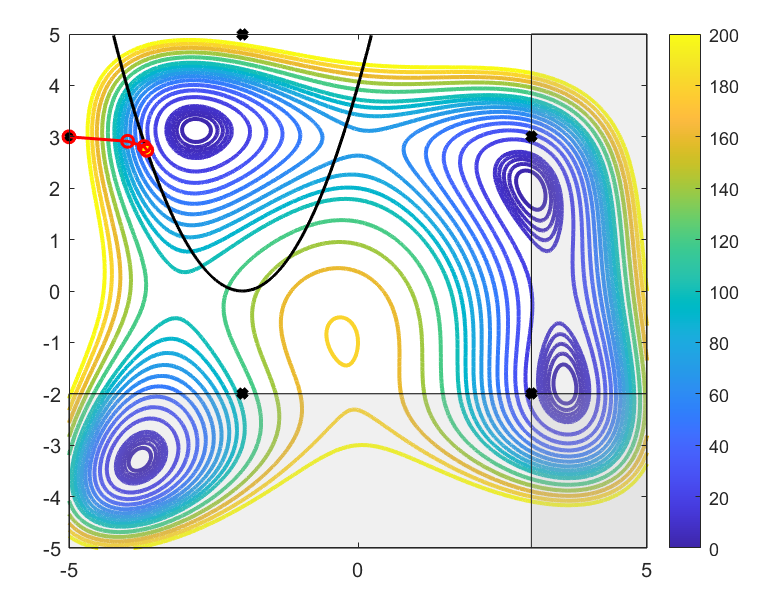
\includegraphics[scale=0.4]{figures/IP_NLP_A.PNG}
%\caption{fig1}
}
\quad
\subfigure[$B(-2,-2)$]{
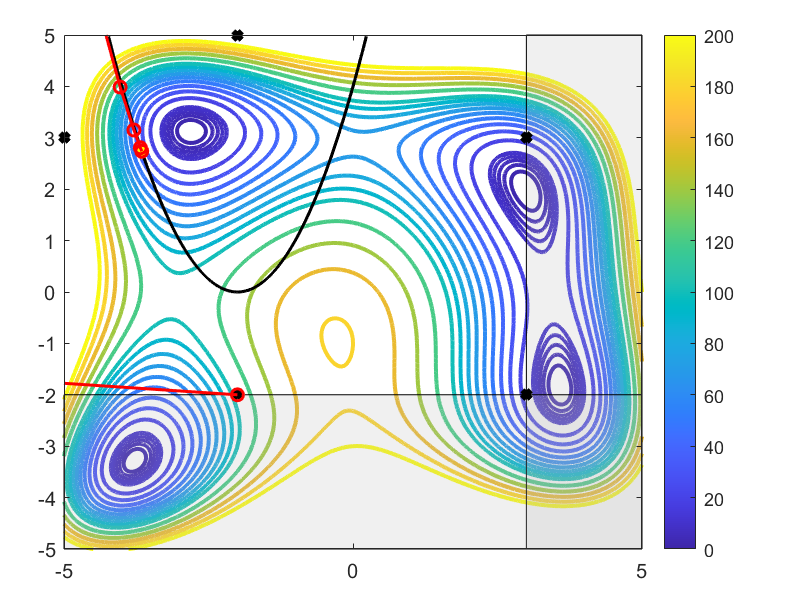
\includegraphics[scale=0.4]{figures/IP_NLP_B.PNG}
}
\quad
\subfigure[$C(3,3)$]{
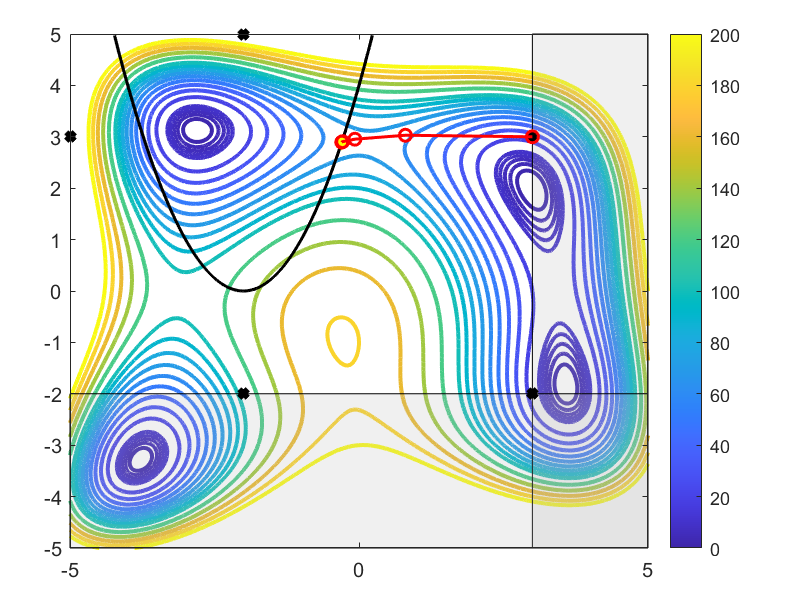
\includegraphics[scale=0.4]{figures/IP_NLP_C.PNG}
}
\quad
\subfigure[$D(-2,5)$]{
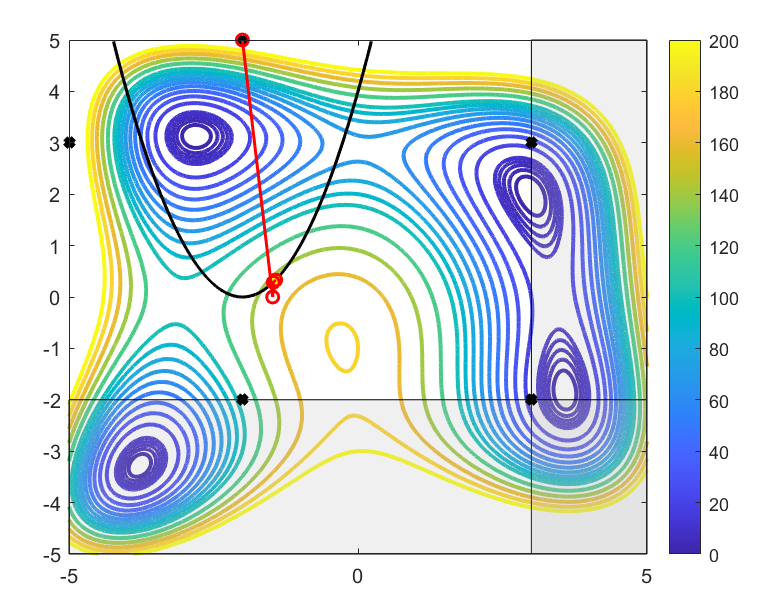
\includegraphics[scale=0.4]{figures/IP_NLP_D.PNG}
}
\quad
\subfigure[$E(3,-2)$]{
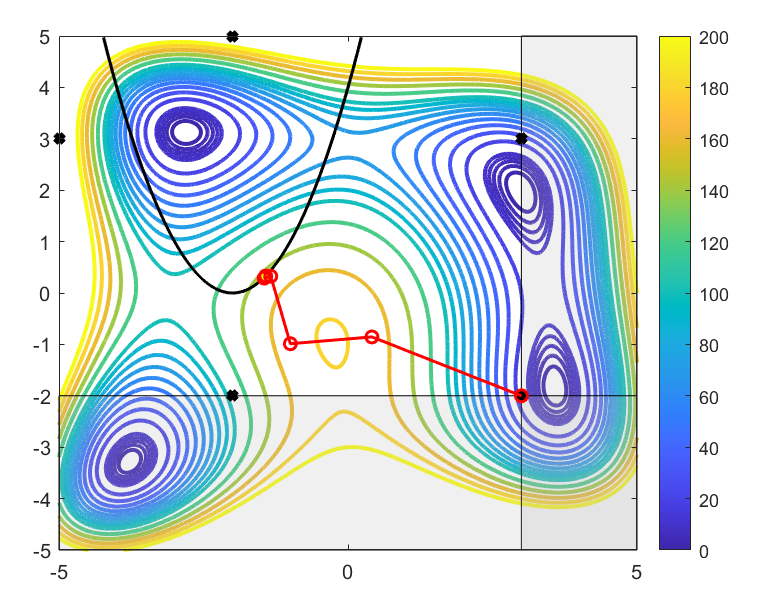
\includegraphics[scale=0.4]{figures/IP_NLP_E.PNG}
}
\caption{ Iterative trajectory in contour}
\end{figure}

%%%%%%%%%%%%%%%%%%%%%%%%%%%%%%%%%%%%%%%%%%%%%%%%%%%%%%%
The iteration of table is showed here separately
%%%%%%%%%%%%%%%%%%%%%%%%%%%%%%%%%%%%%%%%%%%%%%%%%%%%%%
\begin{table}[H]
\centering
\setlength{\abovecaptionskip}{0cm} 
\setlength{\belowcaptionskip}{-0.5cm} 
\scriptsize
\begin{tabular}{|c|c|c|c|c|c|c|c|c|c|}
\hline
$x_0=A(-5,3)$&0&1&2&3&4&5&6&7\\
\hline
$x_1$&-5.0 & -3.99 & -3.7 & -3.66 & -3.66 & -3.66 & -3.65 & -3.65 \\
\hline
$x_2$&3.0 & 2.91 & 2.81 & 2.75 & 2.74 & 2.74 & 2.74 & 2.74
\\
\hline
\end{tabular}
\caption{$x_0=A(-5,3)$}
\end{table}

%%%%%%%%%%%%%%%%%%%%%%%%%%%%%%%%%%%%%%%%%%%%%%%%%%%%%%%%%

%%%%%%%%%%%%%%%%%%%%%%%%%%%%%%%%%%%%%%%%%%%%%%%%%%%%%%%%%
\begin{table}[H]
\centering
\setlength{\abovecaptionskip}{0cm} 
\setlength{\belowcaptionskip}{-0.5cm} 
\scriptsize
\begin{tabular}{|c|c|c|c|c|c|c|c|c|c|c|}
\hline
$x_0=B(-2,-2)$&0&1&2&3&4&5&6&7&8&9\\
\hline
$x_1$&-2.0 & -28.8 & -23.2 & -12.6 & -11.1 & -9.7 & -8.33 & -7.18 & -6.24 & -5.48 \\
\hline
$x_2$&-2.0 & 0 & -1.99 & 1.53 & -1.98 & 57.2 & 38.2 & 25.5 & 17.1 & 11.5
\\
\hline
\end{tabular}

\begin{tabular}{|c|c|c|c|c|c|c|c|c|c|c|}
\hline
$x_0=B(-2,-2)$&10&11&12&13&14&15&16&17&18&19\\
\hline
$x_1$&-4.87 & -4.39 & -4.03 & -3.79 & -3.68 & -3.66 & -3.66 & -3.66 & -3.65 & -3.65   \\
\hline
$x_2$&7.86 & 5.47 & 3.99 & 3.15 & 2.81 & 2.74 & 2.74 & 2.74 & 2.74 & 2.74  
\\
\hline
\end{tabular}
\caption{$x_0=B(-2,-2)$}
\end{table}
%%%%%%%%%%%%%%%%%%%%%%%%%%%%%%%%%%%%%%%%%%%%%%%%%%%%%%%%%%%%%
\begin{table}[H]
\centering
\setlength{\abovecaptionskip}{0cm} 
\setlength{\belowcaptionskip}{-0.5cm} 
\scriptsize
\begin{tabular}{|c|c|c|c|c|c|c|c|c|}
\hline
$x_0=C(3,3)$&0&1&2&3&4&5&6&7\\
\hline
$x_1$&3.0 & 0.803 & -0.0717 & -0.282 & -0.298 & -0.298 & -0.298 & -0.298 \\
\hline
$x_2$&3.0 & 3.03 & 2.95 & 2.91 & 2.9 & 2.9 & 2.9 & 2.9  
\\
\hline
\end{tabular}

\caption{$x_0=C(3,3)$}
\end{table}
%%%%%%%%%%%%%%%%%%%%%%%%%%%%%%%%%%%%%%%%%%%%%%%%%%%%%%%%%%%%%%%
\begin{table}[H]
\centering
\setlength{\abovecaptionskip}{0cm} 
\setlength{\belowcaptionskip}{-0.5cm} 
\scriptsize
\begin{tabular}{|c|c|c|c|c|c|c|c|c|}
\hline
$x_0=D(-2,5)$&0&1&2&3&4&5&6&7\\
\hline
$x_1$&-2.0 & -1.48 & -1.47 & -1.42 & -1.43 & -1.43 & -1.42 & -1.42   \\
\hline
$x_2$&5.0 & 0 & 0.285 & 0.33 & 0.33 & 0.33 & 0.331 & 0.331
\\
\hline
\end{tabular}
\caption{$x_0=D(-2,5)$}
\end{table}
%%%%%%%%%%%%%%%%%%%%%%%%%%%%%%%%%%%%%%%%%%%%%%%%%%%%%%%%%%%
\begin{table}[H]
\centering
\setlength{\abovecaptionskip}{0cm} 
\setlength{\belowcaptionskip}{-0.5cm} 
\scriptsize
\begin{tabular}{|c|c|c|c|c|c|c|c|c|c|c|}
\hline
$x_0=E(3,-2)$&0&1&2&3&4&5&6&7&8&9\\
\hline
$x_1$&3.0 & 0.415 & -0.997 & -1.34 & -1.45 & -1.43 & -1.43 & -1.43 & -1.42 & -1.42 \\
\hline
$x_2$&-2.0 & -0.855 & -0.987 & 0.326 & 0.289 & 0.33 & 0.33 & 0.33 & 0.331 & 0.331 
\\
\hline
\end{tabular}

\caption{$x_0=E(3,-2)$}
\end{table}
It can be seen that starting points $A$ and $B$ have reached the correct minimum points, but starting points $C$ reached a sub-minimum point, and the starting points $D$ and $E$ reached a sub-minimum.\\
First of all, based on the analysis in the previous chapter, it is inferred that the starting points $A$, $B$, and $C$ are the correct iteration trajectories, where the starting point $B$ has many iterations and oscillations, which is related to the choice of step size.
Observing the iterative trajectory of the starting point $D$, it is also speculated that $D$ also jumped directly to a region far away from the correct minimum point because of the too long step size, and instead found the sub-minimum point that meets the convergence condition,
The point E is to approximate the equality constraint curve , and directly passes through the area where the maximum value is located, and also finds the sub-minimum point that meets the convergence condition.

%%%%%%%%%%%%%%%%%%%%%%%%%%%%%%%%%%%%%%%%%%
%%%%%%%%%%%%%%%%%%%%%%%%%%%%%%%%%%%%%%%%%%%
%%%%%%%%%%%%%%%%%%%%%%%%%%%%%%%%%%%%%%%%%%
%%%%%%%%%%%%%%%%%%%%%%%%%%%%%%%%%%%%%%%%%%%
%%%%%%%%%%%%%%%%%%%%%%%%%%%%%%%%%%%%%%%%%%
%%%%%%%%%%%%%%%%%%%%%%%%%%%%%%%%%%%%%%%%%%%
\newpage
\subsection{\bfseries Comparison of algorithms}
\begin{shaded}
{Question:Discuss the different algorithms, the performance of the different algorithms, and
your implementations. In general provide any comments and discussion that
demonstrates that you have an excellent overview of nonlinear programing}
\end{shaded}
First, three methods in the SQP algorithm will be discussed. First the SQP algorithm with damped BFGS and SQP algorithm with damped BFGS and line search are compared. Regardless of whether the step size is limited or not based on line search, these two methods use Newton's method, which is to solve the quadratic programming problem of Taylor quadratic expansion at the current point to determine a search direction, but the method based on line search Finding an optimal step size along this direction makes the objective function drop the most at this step size. It can be seen from the test results of the two algorithms that the method based on line search has fewer iterations, and it can be seen from the iterative curve that the iteration point is easy to produce a larger number based on the Newton method without restricting the step size Jump and oscillate and increase the number of iterations.  Both methods are easy to fall into the local minimum. Compared with this, the SQP method based on the trust region has better performance.\\

In each iteration of the trust region method, first determine a radius of the trust region, and then calculate the minimum value of the second-order approximation of the objective function within the radius. If the minimum value makes the objective function achieve a sufficient decline, then enter the next iteration and expand the radius of the trust region. If the minimum value cannot make the objective function obtain a sufficient decline, it means that the current order of trust region The approximation is not reliable enough, it is necessary to reduce the radius of the trust region and recalculate the minimum value. In the usual nonlinear problem, taking the test problem selected this time as an example, it can be seen that the objective function has four local minimum and one local maximum. If the second-order approximation of the objective function at the current point is close to a local minimum point and is very different from the global minimum point, the line-based search method will find the local minimum point, but the trust region method is reasonably selected In the case of the radius of the trust region, the step size can be controlled more reasonably until the global minimum point is found to achieve a better result. As can be seen from the test results of the algorithm, the iterative curve path based on the trust region is shorter, and there are no unnecessary oscillations and jumps, and the number of iterations is also less. \\

On the formulation of the quadratic subproblem, the IQP approach is used in SQP algorithm with damped BFGS and SQP algorithm with damped BFGS and line search. Because the test question designed here has only two variables, it cannot reflect the high expense of solving the general quadratic subproblem when the nonlinear problem is large. In contrast,in the trust region-based method, the S$l1$QP approach which is an example of EQP method is used to move the linearized constraints into the objective of the quadratic program in the form of an $l1$ penalty term.  The EQP method can have less expense than IQP method in the large-scale cases. Then the S$l1$QP approach further not only can overcome the possible inconsistency among the linearized constraints, but it also ensures that the trust region constraint can always be satisfied.\\

The interior point method implemented in this report is the basic interior point method. A step selection method is used such as line search and trust domain implemented in SQP, so the test results obtained are slightly worse than expected.
Both the continuous method and the obstacle method are applied. The KKT condition of the original problem is converted to the prime-dual system, and gradually change the barrier parameter $\mu$ to search for a central path to gradually optimize the original problem. Among them, the continuous method defines and finds the iterative direction of the prime-dual system. The barrier method guarantees the convergence of the global iteration by moving the barrier parameter to 0. For the update of the barrier parameter, the Fiacco-McCormick approach is used to make the barrier parameter limited to 0. Although this method can achieve good results in most cases, in some cases the choice of the initial point, the initial barrier parameter value, and the scaling of the problem can make problem vulnerable. In order to increase the robustness for all situations, the Adaptive strategies \cite{NoceWrig06} is recommended.\\

Compare SQP with the interior point method. First, SQP is applicable when the number of constraints and the number of variables is very close, because expense can be saved in the formulation and solution of sub-problem in each step. In contrast, the sub-problem solved by each iteration of the interior point method is the same, so it is possible to save iteration expense by optimizing the formulation of the sub-problem. Moreover, because the interior point method iterates within the feasible region, it does not consider all constraints in each iteration, but removes constraints that are not related to the optimal solution, saving iteration costs. Finally, the SQP shows better robustness on badly scaled problems than the nonlinear interior point method.

